\newpage
\section{Specifica Front-End}

\subsection{APIM::FrontEnd}

\subsubsection{Informazioni generali}

\begin{figure}[H]
	\centering
	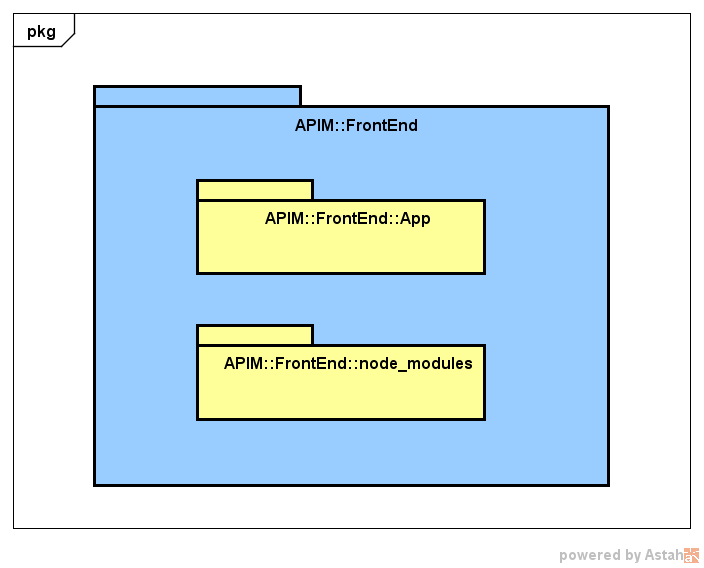
\includegraphics
	[width=0.7\linewidth]
	{images/APIM/FrontEnd/FrontEnd.png}
	\caption{APIM::FrontEnd}
\end{figure}

\begin{itemize}
	\item \textbf{Descrizione:} package contenente le componenti del lato front-end dell'applicazione web;
	\item \textbf{Packages contenuti:}
	\begin{itemize}
		\item App;
		\item node\_modules.
	\end{itemize}
\end{itemize}

\subsection{APIM::FrontEnd::App}

\subsubsection{Informazioni generali}

\begin{figure}[H]
	\centering
	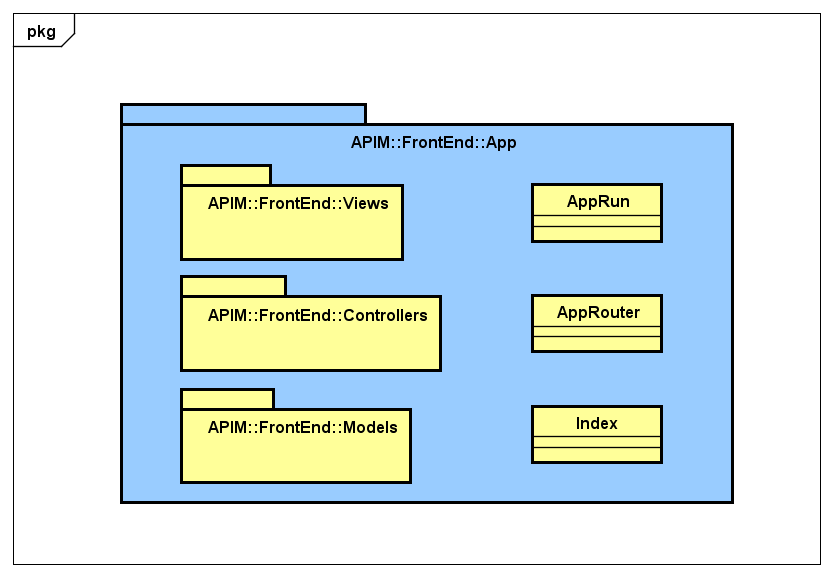
\includegraphics
	[width=0.7\linewidth]
	{images/APIM/FrontEnd/App.png}
	\caption{APIM::FrontEnd::App}
\end{figure}

\begin{itemize}
	\item \textbf{Descrizione:} Il package App contiene tutto il necessario al funzionamento del front-end dell'applicazione web API Market;
	\item \textbf{Packages contenuti:}
	\begin{itemize}
		\item Views;
		\item Models;
		\item Controllers.
	\end{itemize}
\end{itemize}

\subsubsection{Classi}

\paragraph{APIM::FrontEnd::App::AppRouter}

\begin{figure}[H]
	\centering
	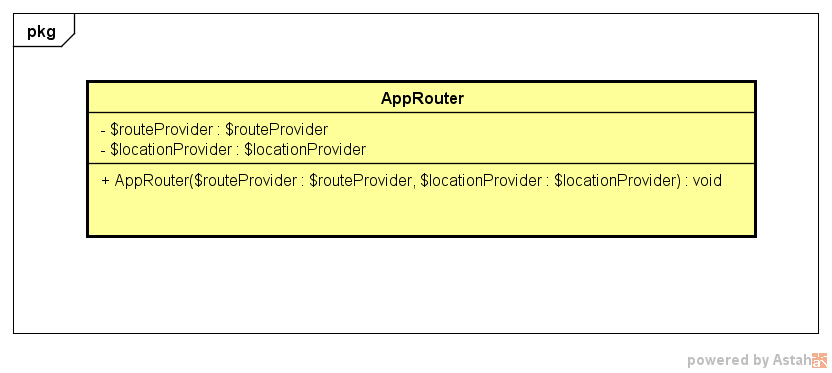
\includegraphics
	[width=0.7\linewidth]
	{images/APIM/FrontEnd/AppRouter.png}
	\caption{APIM::FrontEnd::App::AppRouter}
\end{figure}

\begin{itemize}
	\item \textbf{Descrizione:} La classe AppRouter gestisce le routes dell'applicazione, collegando le views con i rispettivi controllers attraverso i servizi di \$routeProvider e \$locationProvider;
	\item \textbf{Attributi:}
		\begin{itemize}
			\item \textbf{\$routeProvider:} \$routeProvider\\
			Campo dati con il riferimento al servizio di AngularJS dedicato al routing;
			\item \textbf{\$locationProvider:} \$locationProvider\\
			Campo dati con il riferimento al servizio di AngularJS dedicato al pathing;
		\end{itemize}
	\item \textbf{Metodi:}
		\begin{itemize}
			\item \textbf{AppRouter(\$routeProvider: \$routeProvider, \$locationProvider:
\$locationProvider):}
			Metodo per la gestione di routing e pathing dell'applicazione.
		\end{itemize}
\end{itemize}

\paragraph{APIM::FrontEnd::App::AppRun}

\begin{figure}[H]
	\centering
	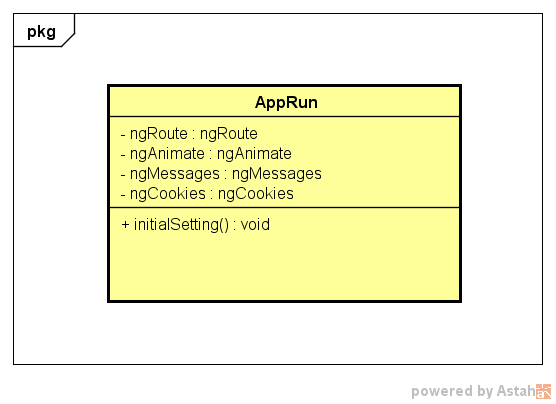
\includegraphics
	[width=0.7\linewidth]
	{images/APIM/FrontEnd/AppRun.png}
	\caption{APIM::FrontEnd::App::AppRun}
\end{figure}

\begin{itemize}
	\item \textbf{Descrizione:} La classe AppRun verifica la corretta autenticazione dell'utente e che le sue autorizzazioni gli consentano di visitare la pagina richiesta;
	\item \textbf{Attributi:}
		\begin{itemize}
			\item \textbf{ngRoute}: ngRoute\\
			Campo dati con il riferimento al modulo ngRoute di AngularJS;
			\item \textbf{ngAnimate}: ngAnimate\\
			Campo dati con il riferimento al modulo ngAnimate di AngularJS;
			\item \textbf{ngMessages}: ngMessages\\
			Campo dati con il riferimento al modulo ngMessages di AngularJS;
			\item \textbf{ngCookies}: ngCookies\\
			Campo dati con il riferimento al modulo ngCookies di AngularJS.
		\end{itemize}
	\item \textbf{Metodi:}
		\begin{itemize}
			\item \textbf{initialSetting(): void}
			Metodo per l'inizializzazione dei campi dati ai valori di default.
		\end{itemize}
	\item \textbf{Relazioni con altre classi:}
	\begin{itemize}
		\item Utilizza il modulo ngRoute per effettuare il routing dell'applicazione;
		\item Utilizza il modulo ngAnimate per impiegare transizioni ed animazioni nell'applicazione;
		\item Utilizza il modulo ngMessages per mostrare messaggi d'aiuto durante le procedure e form dell'applicazione;
		\item Utilizza il modulo ngCookies per effettuare il salvataggio dei cookies dell'applicazione.
	\end{itemize}
\end{itemize}

\paragraph{APIM::FrontEnd::App::Index}

\begin{figure}[H]
	\centering
	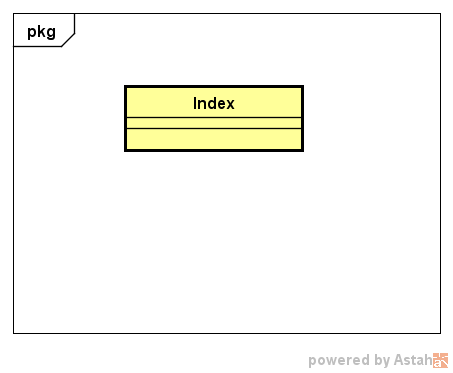
\includegraphics
	[width=0.7\linewidth]
	{images/APIM/FrontEnd/Index.png}
	\caption{APIM::FrontEnd::App::Index}
\end{figure}

\begin{itemize}
	\item \textbf{Descrizione:} La classe Index contiene la view principale dell'applicazione, dove l'utente visualizza dinamicamente le pagine che vuole visitare.
	\item \textbf{Relazioni con altre classi:}
	\begin{itemize}
		\item Interagisce con il package Views, necessario alla corretta visualizzazione delle pagine.
	\end{itemize}
\end{itemize}

% Fine App

\subsection{APIM::FrontEnd::App::Views}

\subsubsection{Informazioni generali}

\begin{figure}[H]
	\centering
	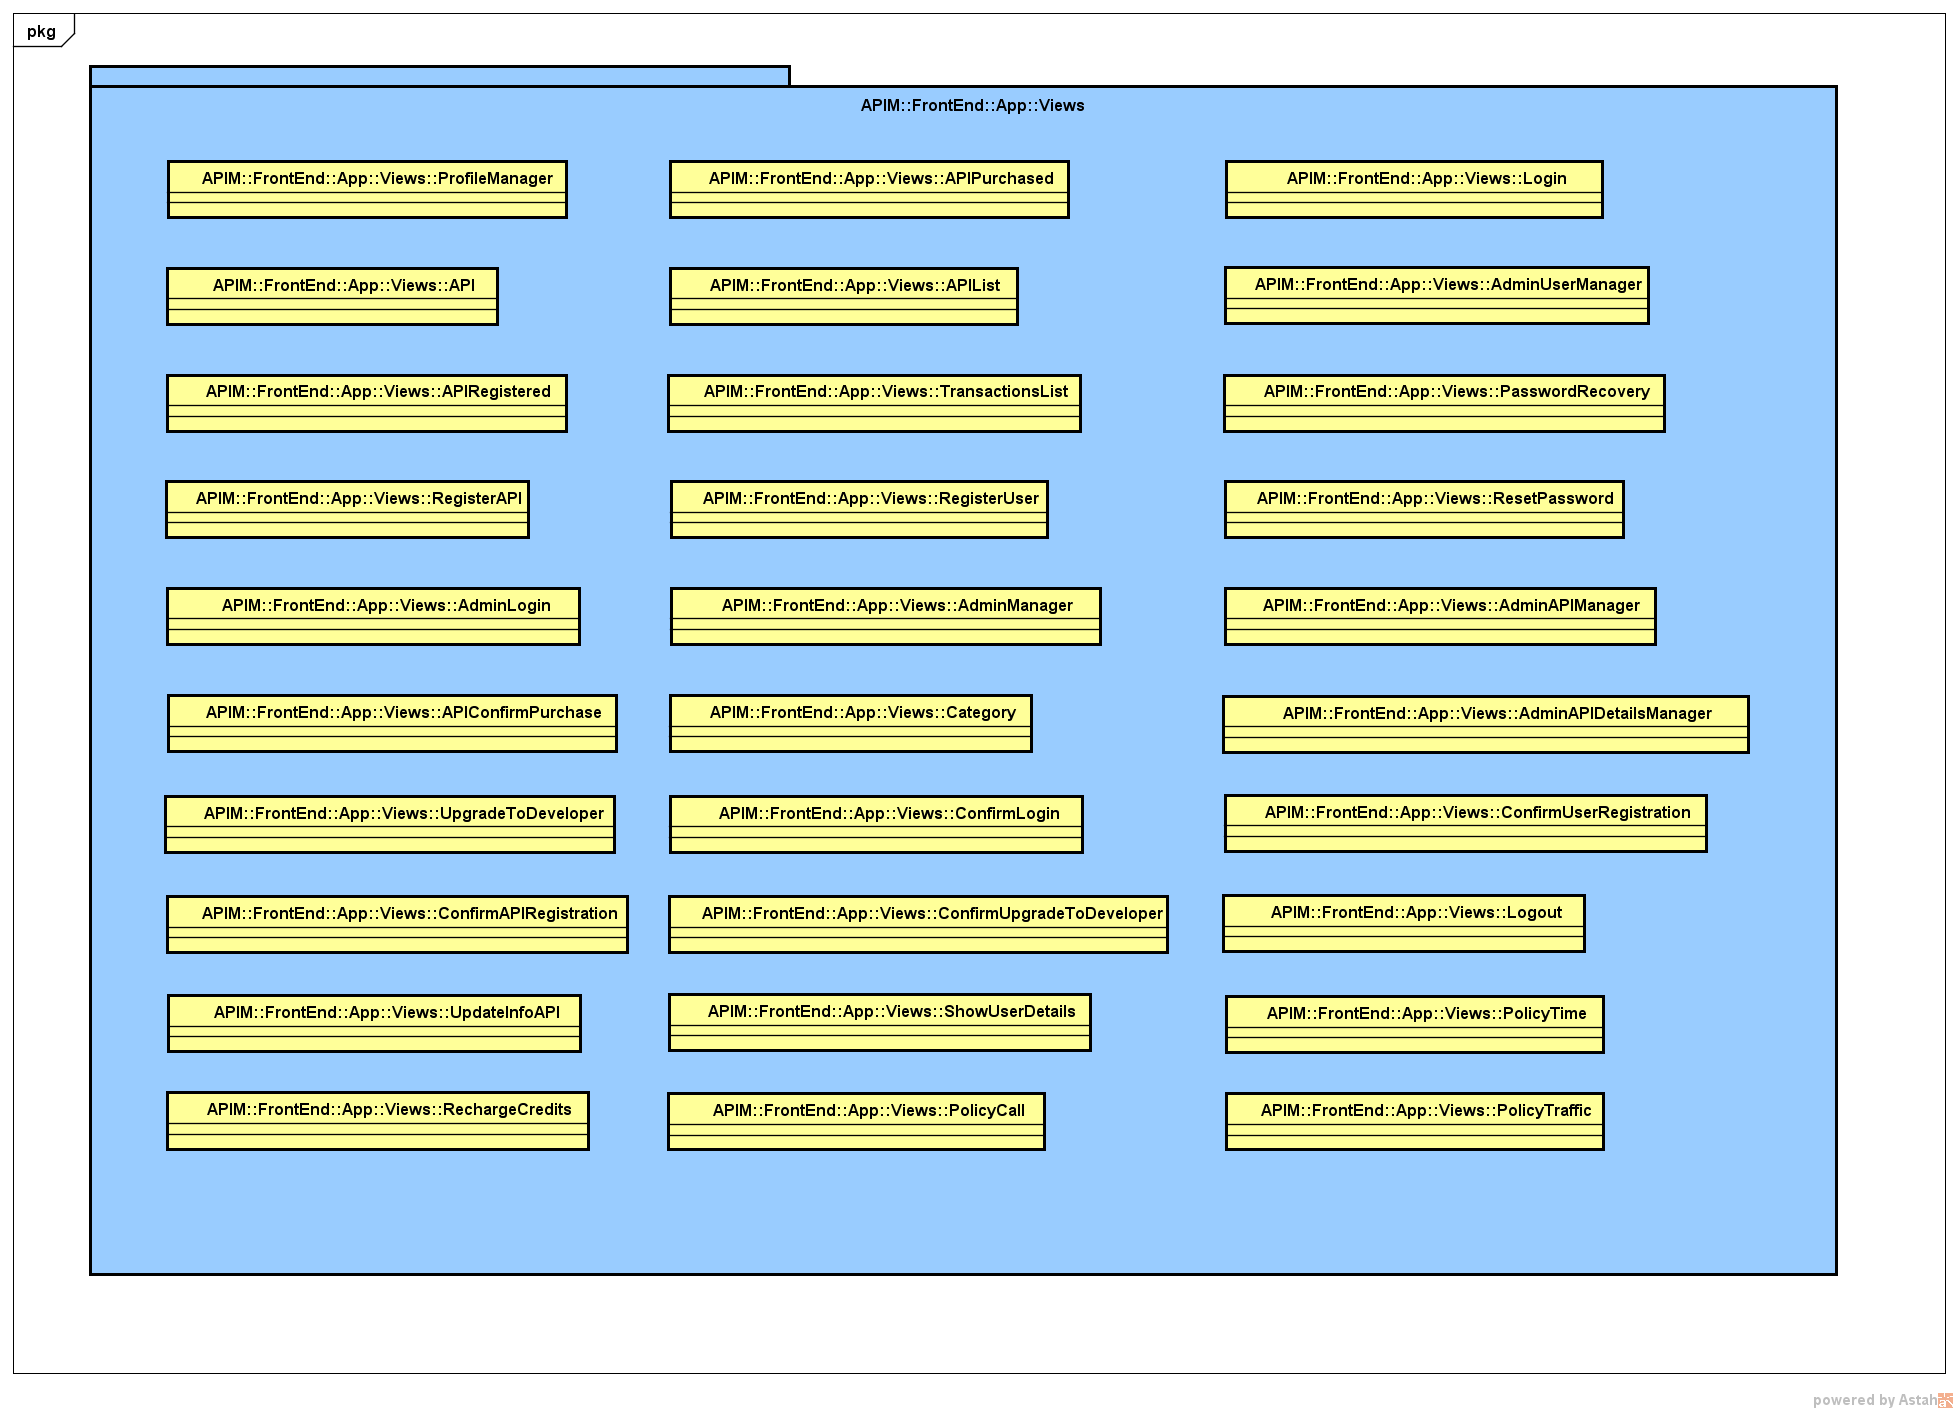
\includegraphics
	[width=0.7\linewidth]
	{images/APIM/FrontEnd/Views/Views.png}
	\caption{APIM::FrontEnd::App::Views}
\end{figure}

\begin{itemize}
	\item \textbf{Descrizione:} Il package Views contiene tutte le view dell'applicazione.
	\item \textbf{Relazioni con altre classi:}
	\begin{itemize}
		\item Il package \textbf{Controllers} collega le views ad un controller per gestirne la visualizzazione da parte dell'utente; 
		\item Il package \textbf{Models} definisce le strutture dati utilizzate da views e controllers.
	\end{itemize}
\end{itemize}

\subsubsection{Classi}

\paragraph{APIM::FrontEnd::App::Views::ProfileManager}

\begin{figure}[H]
	\centering
	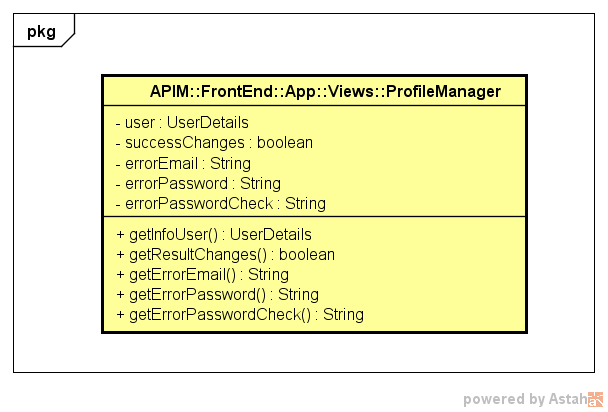
\includegraphics
	[width=0.7\linewidth]
	{images/APIM/FrontEnd/Views/ProfileManager.png}
	\caption{APIM::FrontEnd::App::Views::ProfileManager}
\end{figure}

\begin{itemize}
	\item \textbf{Descrizione:} View contenente le informazioni del profilo personale di un utente registrato. Contiene, inoltre, l'informazione relativa al saldo del proprio conto virtuale;
	\item \textbf{Attributi:}
		\begin{itemize}
			\item \textbf{user : UserDetails}\\
			Campo dati contenente le informazioni di un utente;
			\item \textbf{successChanges : boolean}\\
			Campo dati contenente la conferma delle modifiche;
			\item \textbf{errorEmail : string}\\
			Campo dati contenente l'eventuale errore di inserimento dell'email;
			\item \textbf{errorPassword : string}\\
			Campo dati contenente l'eventuale errore di inserimento della password;
			\item \textbf{errorPasswordCheck : string}\\
			Campo dati contenente l'eventuale errore della conferma della password.
		\end{itemize}
	\item \textbf{Relazioni con altre classi:}
	\begin{itemize}
		\item Interagisce con il controller \textbf{ProfileManagerController};
		\item Il model \textbf{UsersDetailModel} contiene le informazioni per rappresentare un utente.
	\end{itemize}
\end{itemize}

\paragraph{APIM::FrontEnd::App::Views::API}

\begin{figure}[H]
	\centering
	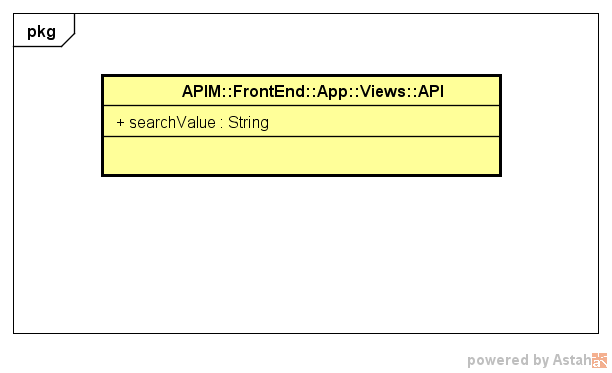
\includegraphics
	[width=0.7\linewidth]
	{images/APIM/FrontEnd/Views/API.png}
	\caption{APIM::FrontEnd::App::Views::API}
\end{figure}

\begin{itemize}
	\item \textbf{Descrizione:} View contenente i risultati della ricerca effettuata, che permette di selezionare un risultato presente al suo interno.
	\item \textbf{Attributi:}
		\begin{itemize}
			\item \textbf{searchContent : string}
			Campo dati contenente le keywords di ricerca dell'API.
		\end{itemize}
	\item \textbf{Relazioni con altre classi:}
	\begin{itemize}
		\item Interagisce con il controller \textbf{APIController};
		\item Il model \textbf{MicroserviceModel} contiene le informazioni per rappresentare una API.
	\end{itemize}
\end{itemize}

\paragraph{APIM::FrontEnd::App::Views::APIRegistered}

\begin{figure}[H]
	\centering
	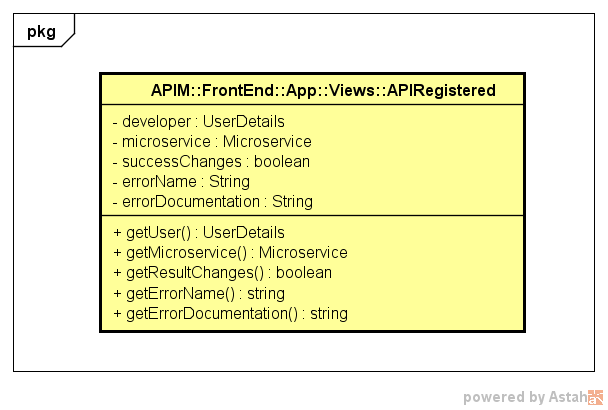
\includegraphics
	[width=0.7\linewidth]
	{images/APIM/FrontEnd/Views/APIRegistered.png}
	\caption{APIM::FrontEnd::App::Views::APIRegistered}
\end{figure}

\begin{itemize}
	\item \textbf{Descrizione:} View contenente la lista delle API registrate dall'utente sulla piattaforma.
	\item \textbf{Attributi:}
		\begin{itemize}
			\item \textbf{developer : UserDetails}\\
			Campo dati contenente le informazioni di un utente sviluppatore;
			\item \textbf{microservice : Microservice}\\
			Campo dati contenente le informazioni di un microservizio;
			\item \textbf{successChanges : boolean}\\
			Campo dati contenente la conferma delle modifiche;
			\item \textbf{errorName : string}\\
			Campo dati contenente l'eventuale errore di inserimento del nome;
			\item \textbf{errorDocumentation: string}\\
			Campo dati contenente l'eventuale errore di inserimento della documentazione.
		\end{itemize}
	\item \textbf{Relazioni con altre classi:}
	\begin{itemize}
		\item Interagisce con il controller \textbf{APIRegisteredController};
		\item Il model \textbf{UsersDetailModel} contiene le informazioni per rappresentare un utente;
		\item Il model \textbf{MicroserviceModel} contiene le informazioni per rappresentare una API.
	\end{itemize}
\end{itemize}

\paragraph{APIM::FrontEnd::App::Views::RegisterAPI}

\begin{figure}[H]
	\centering
	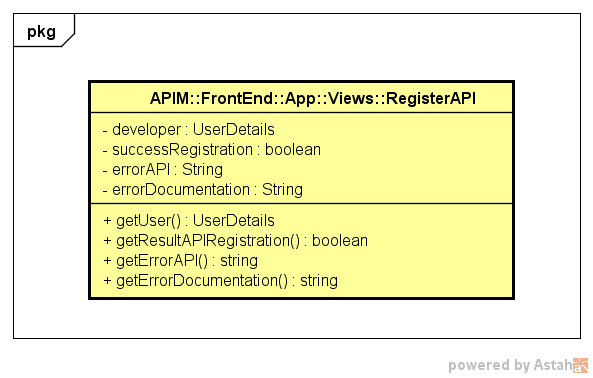
\includegraphics
	[width=0.7\linewidth]
	{images/APIM/FrontEnd/Views/RegisterAPI.png}
	\caption{APIM::FrontEnd::App::Views::RegisterAPI}
\end{figure}

\begin{itemize}
	\item \textbf{Descrizione:} View contenente il form per l'inserimento di una API da parte di un utente sviluppatore. Lo sviluppatore può inserire tutti i dati relativi al microservizio che intende esporre sul marketplace.
	\item \textbf{Attributi:}
		\begin{itemize}
			\item \textbf{developer : UserDetails}\\
			Campo dati contenente le informazioni di un utente sviluppatore;
			\item \textbf{successRegistration : boolean}\\
			Campo dati contenente la conferma della registrazione;
			\item \textbf{errorAPI : string}\\
			Campo dati contenente l'eventuale errore di inserimento dell'API;
			\item \textbf{errorDocumentation: string}\\
			Campo dati contenente l'eventuale errore di inserimento della documentazione.
		\end{itemize}
	\item \textbf{Relazioni con altre classi:}
	\begin{itemize}
		\item Interagisce con il controller \textbf{RegisterAPIController};
		\item Il model \textbf{UsersDetailModel} contiene le informazioni per rappresentare un utente;
		\item Il model \textbf{MicroserviceModel} contiene le informazioni per rappresentare una API.
	\end{itemize}
\end{itemize}

\paragraph{APIM::FrontEnd::App::Views::PolicyCall}

\begin{figure}[H]
	\centering
	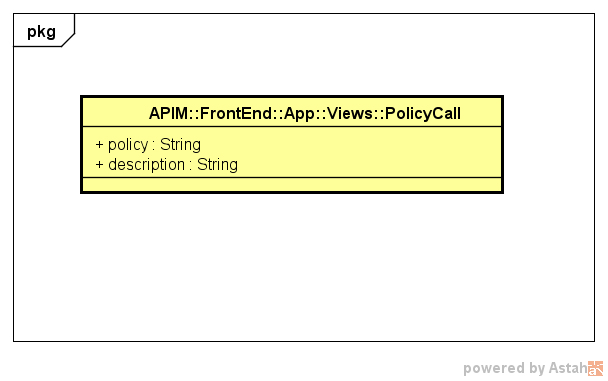
\includegraphics
	[width=0.7\linewidth]
	{images/APIM/FrontEnd/Views/PolicyCall.png}
	\caption{APIM::FrontEnd::App::Views::PolicyCall}
\end{figure}

\begin{itemize}
	\item \textbf{Descrizione:} View contenente le informazioni relative alla policy per chiamate.
	\item \textbf{Attributi:}
		\begin{itemize}
			\item \textbf{policy : string}\\
			Campo dati contenente la policy di una API;
			\item \textbf{description : string}\\
			Campo dati contenente la descrizione di una policy a chiamate.
		\end{itemize}
	\item \textbf{Relazioni con altre classi:}
	\begin{itemize}
		\item Interagisce con il controller \textbf{PolicyCallController};
		\item Il model \textbf{MicroserviceModel} contiene le informazioni per rappresentare una API.
	\end{itemize}
\end{itemize}

\paragraph{APIM::FrontEnd::App::Views::PolicyTime}

\begin{figure}[H]
	\centering
	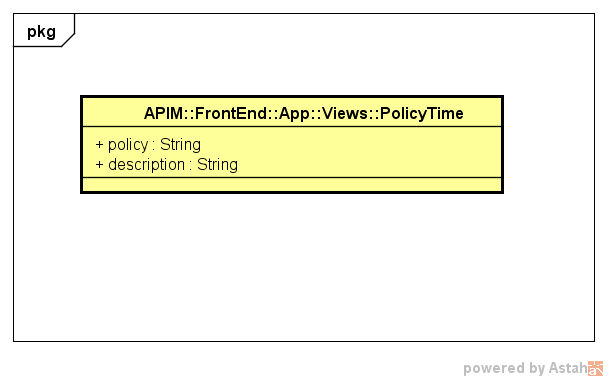
\includegraphics
	[width=0.7\linewidth]
	{images/APIM/FrontEnd/Views/PolicyTime.png}
	\caption{APIM::FrontEnd::App::Views::PolicyTime}
\end{figure}

\begin{itemize}
	\item \textbf{Descrizione:} View contenente le informazioni relative alla policy per tempo.
	\item \textbf{Attributi:}
	\begin{itemize}
		\item \textbf{policy : string}\\
		Campo dati contenente la policy di una API;
		\item \textbf{description : string}\\
		Campo dati contenente la descrizione di una policy a tempo.
	\end{itemize}
	\item \textbf{Relazioni con altre classi:}
	\begin{itemize}
		\item Interagisce con il controller \textbf{PolicyTimeController};
		\item Il model \textbf{MicroserviceModel} contiene le informazioni per rappresentare una API.
	\end{itemize}
\end{itemize}

\paragraph{APIM::FrontEnd::App::Views::PolicyTraffic}

\begin{figure}[H]
	\centering
	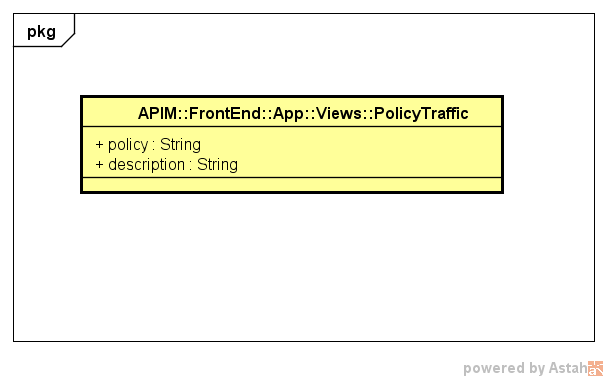
\includegraphics
	[width=0.7\linewidth]
	{images/APIM/FrontEnd/Views/PolicyTraffic.png}
	\caption{APIM::FrontEnd::App::Views::PolicyTraffic}
\end{figure}

\begin{itemize}
	\item \textbf{Descrizione:} View contenente le informazioni relative alla policy per traffico dati.
	\item \textbf{Attributi:}
	\begin{itemize}
		\item \textbf{policy : string}\\
		Campo dati contenente la policy di una API;
		\item \textbf{description : string}\\
		Campo dati contenente la descrizione di una policy per traffico.
	\end{itemize}
	\item \textbf{Relazioni con altre classi:}
	\begin{itemize}
		\item Interagisce con il controller \textbf{PolicyTrafficController};
		\item Il model \textbf{MicroserviceModel} contiene le informazioni per rappresentare una API.
	\end{itemize}
\end{itemize}

\paragraph{APIM::FrontEnd::App::Views::APIPurchased}

\begin{figure}[H]
	\centering
	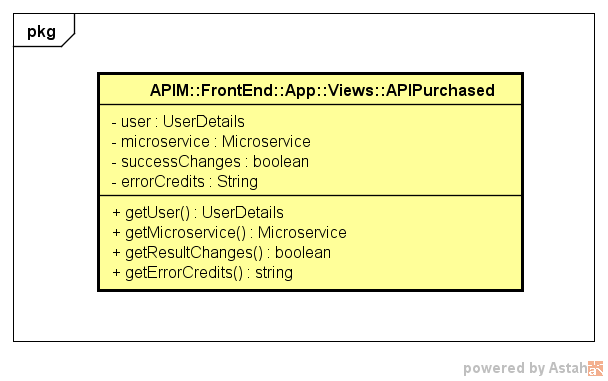
\includegraphics
	[width=0.7\linewidth]
	{images/APIM/FrontEnd/Views/APIPurchased.png}
	\caption{APIM::FrontEnd::App::Views::APIPurchased}
\end{figure}

\begin{itemize}
	\item \textbf{Descrizione:} View contenente la lista delle API acquistate da un utente della piattaforma API Market.
	\item \textbf{Attributi:}
		\begin{itemize}
			\item \textbf{user : UserDetails}\\
			Campo dati contenente le informazioni di un utente;
			\item \textbf{microservice : Microservice}\\
			Campo dati contenente le informazioni di una API;
			\item \textbf{successChanges : boolean}\\
			Campo dati contenente la conferma del rinnovo dell'API;
			\item \textbf{errorCredits : string}\\
			Campo dati contenente l'eventuale errore di rinnovo dell'API.
		\end{itemize}
	\item \textbf{Relazioni con altre classi:}
	\begin{itemize}
		\item Interagisce con il controller \textbf{APIPurchasedController};
		\item Il model \textbf{UserDetailsModel} contiene le informazioni per rappresentare un utente;
		\item Il model \textbf{TransactionModel} contiene le informazioni per rappresentare una transazione;
		\item Il model \textbf{MicroserviceModel} contiene le informazioni per rappresentare una API.
	\end{itemize}
\end{itemize}

\paragraph{APIM::FrontEnd::App::Views::APIList}

\begin{figure}[H]
	\centering
	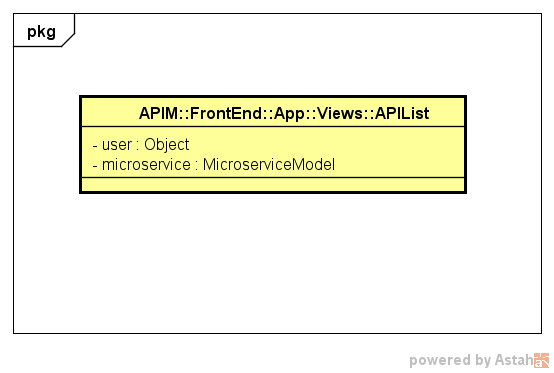
\includegraphics
	[width=0.7\linewidth]
	{images/APIM/FrontEnd/Views/APIList.png}
	\caption{APIM::FrontEnd::App::Views::APIList}
\end{figure}

\begin{itemize}
	\item \textbf{Descrizione:} View contenente l'elenco delle API disponibili sul marketplace \progetto.
	\item \textbf{Attributi:}
	\begin{itemize}
		\item \textbf{user : UserDetails}\\
		Campo dati contenente le informazioni di un utente;
		\item \textbf{microservice : Microservice}\\
		Campo dati contenente le informazioni di una API.
	\end{itemize}
	\item \textbf{Relazioni con altre classi:}
	\begin{itemize}
		\item Interagisce con il controller \textbf{APIListController};
		\item Il model \textbf{UserDetailsModel} contiene le informazioni per rappresentare un utente;
		\item Il model \textbf{MicroserviceModel} contiene le informazioni per rappresentare una API.
	\end{itemize}
\end{itemize}

\paragraph{APIM::FrontEnd::App::Views::TransactionsList}

\begin{figure}[H]
	\centering
	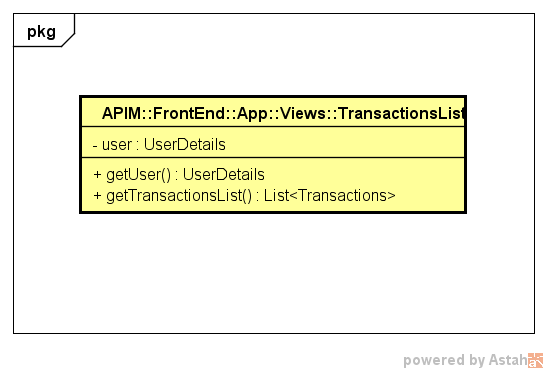
\includegraphics
	[width=0.7\linewidth]
	{images/APIM/FrontEnd/Views/TransactionsList.png}
	\caption{APIM::FrontEnd::App::Views::TransactionsList}
\end{figure}

\begin{itemize}
	\item \textbf{Descrizione:} View contenente l'elenco delle transazioni effettuate da un utente
su API Market.
	\item \textbf{Attributi:}
	\begin{itemize}
		\item \textbf{user : UserDetails}\\
		Campo dati contenente le informazioni di un utente.
		\item \textbf{transactions : List<Transaction>}\\
		Campo dati contenente la lista delle transazioni di un utente.
	\end{itemize}
	\item \textbf{Relazioni con altre classi:}
	\begin{itemize}
		\item Interagisce con il controller \textbf{TransactionsListController};
		\item Il model \textbf{TransactionModel} contiene le informazioni per rappresentare una API.
	\end{itemize}
\end{itemize}

\paragraph{APIM::FrontEnd::App::Views::RegisterUser}

\begin{figure}[H]
	\centering
	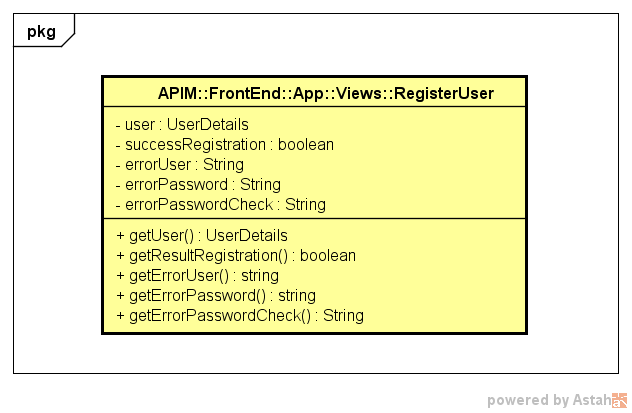
\includegraphics
	[width=0.7\linewidth]
	{images/APIM/FrontEnd/Views/RegisterUser.png}
	\caption{APIM::FrontEnd::App::Views::RegisterUser}
\end{figure}

\begin{itemize}
	\item \textbf{Descrizione:} View contenente il form dedicato alla registrazione di un utente, il
quale può inserire i campi necessari e registrarsi così alla piattaforma. Contiene,
inoltre, un link alla pagina di login;
	\item \textbf{Attributi:}
	\begin{itemize}
		\item \textbf{user : UserDetails}\\
		Campo dati contenente le informazioni di un utente;
		\item \textbf{successRegistration : boolean}\\
		Campo dati contenente il flag di successo della registrazione;
		\item \textbf{errorUser : string}\\
		Campo dati contenente l'eventuale errore di inserimento delle informazioni dell'utente;
		\item \textbf{errorPassword : string}\\
		Campo dati contenente l'eventuale errore di inserimento della password;
		\item \textbf{errorPasswordCheck : string}\\
		Campo dati contenente l'eventuale errore di reinserimento della password.
	\end{itemize}
	\item \textbf{Relazioni con altre classi:}
	\begin{itemize}
		\item Interagisce con il controller \textbf{RegisterUserController};
		\item Il model \textbf{UserDetailsModel} contiene le informazioni per rappresentare un utente.
	\end{itemize}
\end{itemize}

\paragraph{APIM::FrontEnd::App::Views::AdminManager}

\begin{figure}[H]
	\centering
	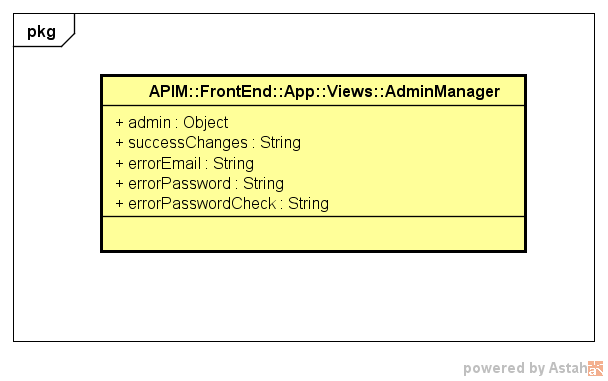
\includegraphics
	[width=0.7\linewidth]
	{images/APIM/FrontEnd/Views/AdminManager.png}
	\caption{APIM::FrontEnd::App::Views::AdminManager}
\end{figure}

\begin{itemize}
	\item \textbf{Descrizione:} View contenente le operazioni per la gestione del profilo amministratore
API Market.
	\item \textbf{Attributi:}
	\begin{itemize}
		\item \textbf{admin : UserAdmin}\\
		Campo dati contenente le informazioni di un admin;
		\item \textbf{successChanges : boolean}\\
		Campo dati contenente il messaggio di successo delle modifiche;
		\item \textbf{errorEmail : string}\\
		Campo dati contenente l'eventuale errore di inserimento delle informazioni dell'utente;
		\item \textbf{errorPassword : string}\\
		Campo dati contenente l'eventuale errore di inserimento della password;
		\item \textbf{errorPasswordCheck : string}\\
		Campo dati contenente l'eventuale errore di reinserimento della password.
	\end{itemize}
	\item \textbf{Relazioni con altre classi:}
	\begin{itemize}
		\item Interagisce con il controller \textbf{AdminManagerController};
		\item Il model \textbf{UserDetailsModel} contiene le informazioni per rappresentare un utente.
	\end{itemize}
\end{itemize}

\paragraph{APIM::FrontEnd::App::Views::Login}

\begin{figure}[H]
	\centering
	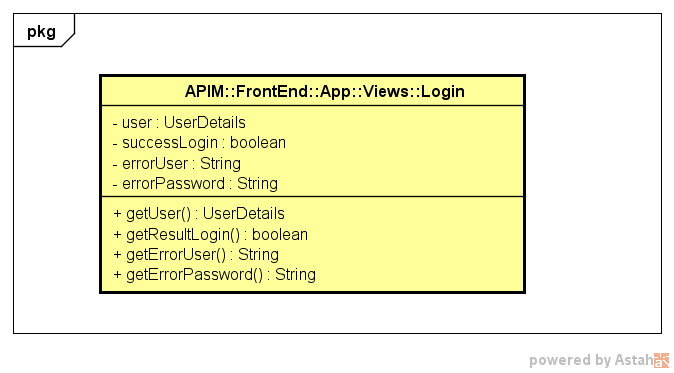
\includegraphics
	[width=0.7\linewidth]
	{images/APIM/FrontEnd/Views/Login.png}
	\caption{APIM::FrontEnd::App::Views::Login}
\end{figure}

\begin{itemize}
	\item \textbf{Descrizione:} View contenente il form necessario affinchè l'utente possa effettuare il login ed autenticarsi al sistema. Contiene, inoltre, un link alla pagina di registrazione e uno alla pagina per il recupero della password
	\item \textbf{Attributi:}
	\begin{itemize}
		\item \textbf{user : UserDetails}\\
		Campo dati contenente le informazioni di un utente;
		\item \textbf{successLogin : boolean}\\
		Campo dati contenente il messaggio di successo del login;
		\item \textbf{errorUser : string}\\
		Campo dati contenente l'eventuale errore di inserimento delle informazioni dell'utente;
		\item \textbf{errorPassword : string}\\
		Campo dati contenente l'eventuale errore di inserimento della password.
	\end{itemize}
	\item \textbf{Relazioni con altre classi:}
	\begin{itemize}
		\item Interagisce con il controller \textbf{LoginController};
		\item Il model \textbf{UserDetailsModel} contiene le informazioni per rappresentare un utente.
	\end{itemize}
\end{itemize}

\paragraph{APIM::FrontEnd::App::Views::AdminAPIDetailsManager}

\begin{figure}[H]
	\centering
	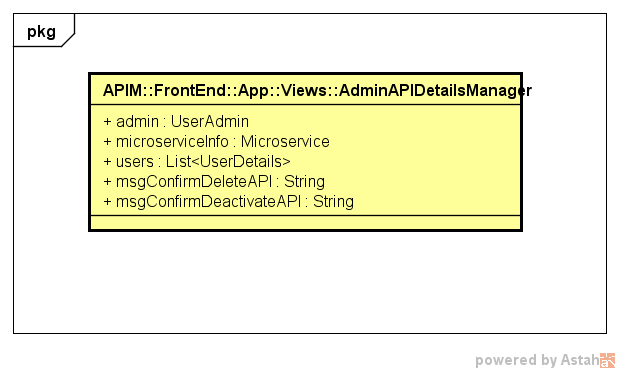
\includegraphics
	[width=0.7\linewidth]
	{images/APIM/FrontEnd/Views/AdminAPIDetailsManager.png}
	\caption{APIM::FrontEnd::App::Views::AdminAPIDetailsManager}
\end{figure}

\begin{itemize}
	\item \textbf{Descrizione:} View contenente le statistiche di una API dell'\progetto.\\
	\item \textbf{Attributi:}
	\begin{itemize}
		\item \textbf{admin : UserAdmin}\\
		Campo dati contenente le informazioni di un admin;
		\item \textbf{microserviceInfo : Microservice}\\
		Campo dati contenente le informazioni di un microservizio;
		\item \textbf{users : List<UserDetails>}\\
		Campo dati contenente la lista degli utenti per una relativa API.
		\item \textbf{msgConfirmDeleteAPI : string}\\
		Campo dati contenente il messaggio di conferma della cancellazione API.
		\item \textbf{msgConfirmDeactivateAPI : string}\\
		Campo dati contenente il messaggio di conferma della disattivazione API.
	\end{itemize}
	\item \textbf{Relazioni con altre classi:}
	\begin{itemize}
		\item Interagisce con il controller \textbf{AdminAPIDetailsManagerController};
		\item Il model \textbf{MicroserviceModel} contiene le informazioni per rappresentare un microservizio.
	\end{itemize}
\end{itemize}

\paragraph{APIM::FrontEnd::App::Views::PasswordRecovery}

\begin{figure}[H]
	\centering
	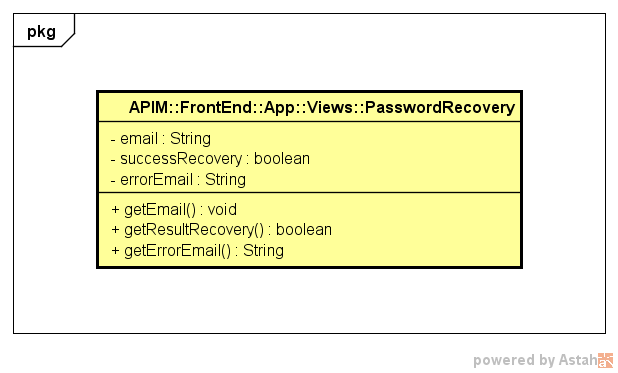
\includegraphics
	[width=0.7\linewidth]
	{images/APIM/FrontEnd/Views/PasswordRecovery.png}
	\caption{APIM::FrontEnd::App::Views::PasswordRecovery}
\end{figure}

\begin{itemize}
	\item \textbf{Descrizione:} View contenente il form dedicato al recupero della password di un utente, il quale può inserire l'indirizzo email e ricevere una nuova password con la quale autenticarsi al sistema. Contiene, inoltre, un link alla pagina di login;
	\item \textbf{Attributi:}
	\begin{itemize}
		\item \textbf{email : string}\\
		Campo dati contenente un indirizzo email;
		\item \textbf{successRecovery : boolean}\\
		Campo dati contenente il flag di successo del recupero password;
		\item \textbf{errorEmail : string}\\
		Campo dati contenente l'eventuale errore di inserimento dell'indirizzo email.
	\end{itemize}
	\item \textbf{Relazioni con altre classi:}
	\begin{itemize}
		\item Interagisce con il controller \textbf{PasswordRecoveryController};
		\item Il model \textbf{UserDetailsModel} contiene le informazioni per rappresentare un utente.
	\end{itemize}
\end{itemize}

\paragraph{APIM::FrontEnd::App::Views::ResetPassword}

\begin{figure}[H]
	\centering
	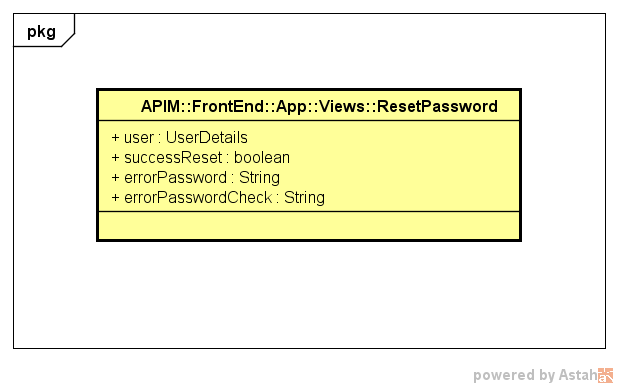
\includegraphics
	[width=0.7\linewidth]
	{images/APIM/FrontEnd/Views/ResetPassword.png}
	\caption{APIM::FrontEnd::App::Views::ResetPassword}
\end{figure}

\begin{itemize}
	\item \textbf{Descrizione:} View contenente il form dedicato al cambio di password di un utente
autenticato, il quale può inserire la nuova password che intende utilizzare per i futuri login al sistema.
	\item \textbf{Attributi:}
	\begin{itemize}
		\item \textbf{user : UserDetails}\\
		Campo dati contenente le informazioni di un utente;
		\item \textbf{successReset : boolean}\\
		Campo dati contenente il flag di successo del reset password;
		\item \textbf{errorPassword : string}\\
		Campo dati contenente l'eventuale errore di inserimento della password.
		\item \textbf{errorPasswordCheck : string}\\
		Campo dati contenente l'eventuale errore di reinserimento della password.
	\end{itemize}
	\item \textbf{Relazioni con altre classi:}
	\begin{itemize}
		\item Interagisce con il controller \textbf{ResetPasswordController};
		\item Il model \textbf{UserDetailsModel} contiene le informazioni per rappresentare un utente.
	\end{itemize}
\end{itemize}

\paragraph{APIM::FrontEnd::App::Views::AdminUserManager}

\begin{figure}[H]
	\centering
	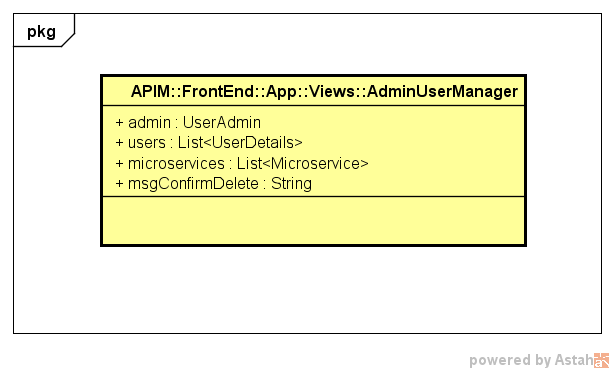
\includegraphics
	[width=0.7\linewidth]
	{images/APIM/FrontEnd/Views/AdminUserManager.png}
	\caption{APIM::FrontEnd::App::Views::AdminUserManager}
\end{figure}

\begin{itemize}
	\item \textbf{Descrizione:} View contenente le operazioni di un ammistratore sugli utenti dell'\progetto.
	\item \textbf{Attributi:}
	\begin{itemize}
		\item \textbf{admin : UserAdmin}\\
		Campo dati contenente le informazioni di un admin;
		\item \textbf{users : List<UserDetails>}\\
		Campo dati contenente la lista di utenti registrati nella piattaforma.
		\item \textbf{microservices : List<Microservice>}\\
		Campo dati contenente la lista dei microservizi registrati per ogni utente.
		\item \textbf{msgConfirmDelete : string}\\
		Campo dati contenente il messaggio di conferma eliminazione
	\end{itemize}
	\item \textbf{Relazioni con altre classi:}
	\begin{itemize}
		\item Interagisce con il controller \textbf{AdminUserManagerController};
		\item Il model \textbf{UserDetailsModel} contiene le informazioni per rappresentare un utente.
		\item Il model \textbf{MicroserviceModel} contiene le informazioni per rappresentare un microservizio.
	\end{itemize}
\end{itemize}

\paragraph{APIM::FrontEnd::App::Views::APIConfirmPurchase}

\begin{figure}[H]
	\centering
	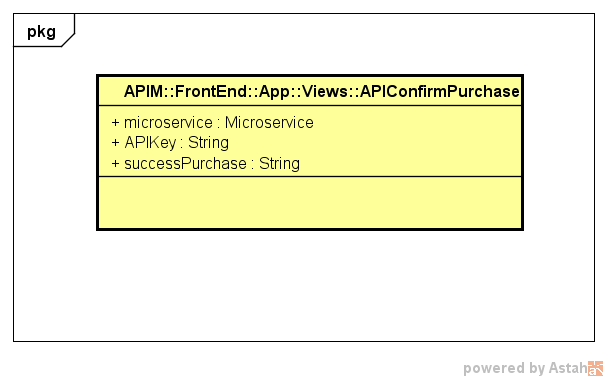
\includegraphics
	[width=0.7\linewidth]
	{images/APIM/FrontEnd/Views/APIConfirmPurchase.png}
	\caption{APIM::FrontEnd::App::Views::APIConfirmPurchase}
\end{figure}

\begin{itemize}
	\item \textbf{Descrizione:} View contenente la conferma di un acquisto di una API.
	\item \textbf{Attributi:}
	\begin{itemize}
		\item \textbf{microservice : Microservice}\\
		Campo dati contenente le informazioni di un microservizio;
		\item \textbf{APIKey : string}\\
		Campo dati contenente l'API key per il microservizio acquistato.
		\item \textbf{successPurchase : string}\\
		Campo dati contenente un messaggio di conferma per l'acquisto.
	\end{itemize}
	\item \textbf{Relazioni con altre classi:}
	\begin{itemize}
		\item Interagisce con il controller \textbf{APIConfirmPurchaseController};
		\item Il model \textbf{MicroserviceModel} contiene le informazioni per rappresentare un microservizio.
	\end{itemize}
\end{itemize}


\paragraph{APIM::FrontEnd::App::Views::Category}

\begin{figure}[H]
	\centering
	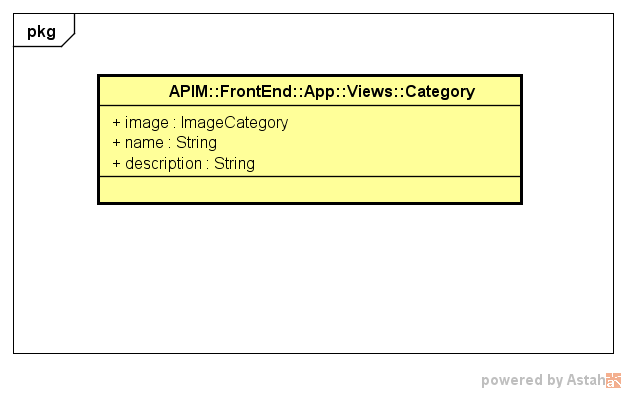
\includegraphics
	[width=0.7\linewidth]
	{images/APIM/FrontEnd/Views/Category.png}
	\caption{APIM::FrontEnd::App::Views::Category}
\end{figure}

\begin{itemize}
	\item \textbf{Descrizione:} View contenente l'elenco delle categorie nell'\progetto
	\item \textbf{Attributi:}
	\begin{itemize}
		\item \textbf{image : ImageCategory}\\
		Campo dati contenente un immagine della categoria;
		\item \textbf{name : string}\\
		Campo dati contenente il nome della categoria;
		\item \textbf{description : string}\\
		Campo dati contenente la descrizione della categoria.
	\end{itemize}
	\item \textbf{Relazioni con altre classi:}
	\begin{itemize}
		\item Interagisce con il controller \textbf{CategoryController};
	\end{itemize}
\end{itemize}

\paragraph{APIM::FrontEnd::App::Views::ConfirmUpgradeToDeveloper}

\begin{figure}[H]
	\centering
	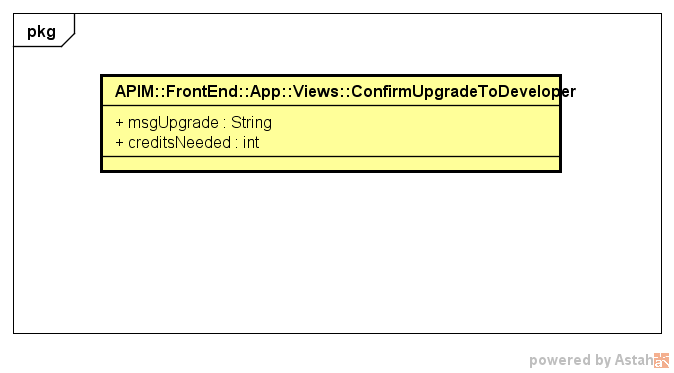
\includegraphics
	[width=0.7\linewidth]
	{images/APIM/FrontEnd/Views/ConfirmUpgradeToDeveloper.png}
	\caption{APIM::FrontEnd::App::Views::ConfirmUpgradeToDeveloper}
\end{figure}

\begin{itemize}
	\item \textbf{Descrizione:} View contenente la conferma dell'upgrade di un utente a sviluppatore nell'\progetto.
	\item \textbf{Attributi:}
	\begin{itemize}
		\item \textbf{msgUpgrade : string}\\
		Campo dati contenente un messaggio per la procedura di upgrade;
		\item \textbf{creditsNeeded : int}\\
		Campo dati contenente il numero di crediti necessari all'upgrade.
	\end{itemize}
	\item \textbf{Relazioni con altre classi:}
	\begin{itemize}
		\item Interagisce con il controller \textbf{ConfirmUpgradeToDeveloperController};
	\end{itemize}
\end{itemize}

\paragraph{APIM::FrontEnd::App::Views::ConfirmLogin}

\begin{figure}[H]
	\centering
	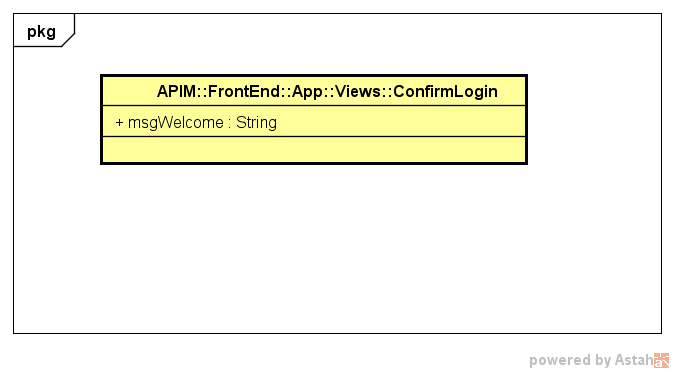
\includegraphics
	[width=0.7\linewidth]
	{images/APIM/FrontEnd/Views/ConfirmLogin.png}
	\caption{APIM::FrontEnd::App::Views::ConfirmLogin}
\end{figure}

\begin{itemize}
	\item \textbf{Descrizione:} View contenente la conferma di login all'\progetto.
	\item \textbf{Attributi:}
	\begin{itemize}
		\item \textbf{msgWelcome : string}\\
		Campo dati contenente un messaggio di benvenuto post autenticazione;
	\end{itemize}
	\item \textbf{Relazioni con altre classi:}
	\begin{itemize}
		\item Interagisce con il controller \textbf{ConfirmLoginController};
	\end{itemize}
\end{itemize}

\paragraph{APIM::FrontEnd::App::Views::ConfirmUserRegistration}

\begin{figure}[H]
	\centering
	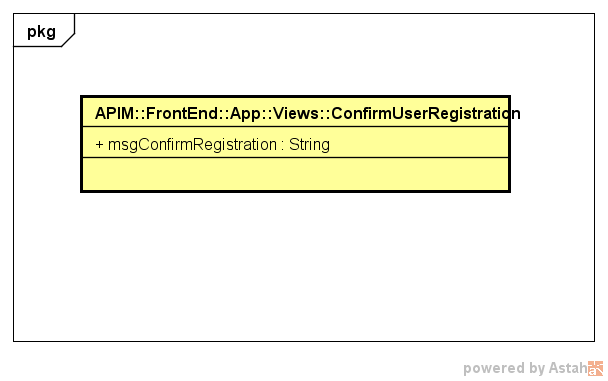
\includegraphics
	[width=0.7\linewidth]
	{images/APIM/FrontEnd/Views/ConfirmUserRegistration.png}
	\caption{APIM::FrontEnd::App::Views::ConfirmUserRegistration}
\end{figure}

\begin{itemize}
	\item \textbf{Descrizione:} View contenente la conferma di registrazione all'\progetto..
	\item \textbf{Attributi:}
	\begin{itemize}
		\item \textbf{msgConfirmRegistration : string}\\
		Campo dati contenente un messaggio di conferma registrazione;
	\end{itemize}
	\item \textbf{Relazioni con altre classi:}
	\begin{itemize}
		\item Interagisce con il controller \textbf{ConfirmUserRegistrationController};
	\end{itemize}
\end{itemize}

\paragraph{APIM::FrontEnd::App::Views::ConfirmAPIRegistration}

\begin{figure}[H]
	\centering
	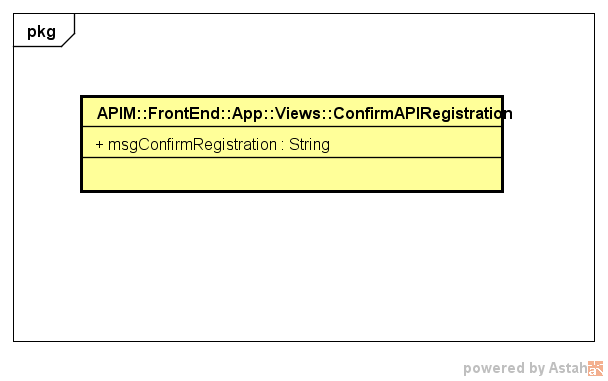
\includegraphics
	[width=0.7\linewidth]
	{images/APIM/FrontEnd/Views/ConfirmAPIRegistration.png}
	\caption{APIM::FrontEnd::App::Views::ConfirmAPIRegistration}
\end{figure}

\begin{itemize}
	\item \textbf{Descrizione:} View contenente la conferma di registrazione di una API all'\progetto.
	\item \textbf{Attributi:}
	\begin{itemize}
		\item \textbf{msgConfirmRegistration : string}\\
		Campo dati contenente un messaggio di conferma registrazione API;
	\end{itemize}
	\item \textbf{Relazioni con altre classi:}
	\begin{itemize}
		\item Interagisce con il controller \textbf{ConfirmAPIRegistrationController};
	\end{itemize}
\end{itemize}

\paragraph{APIM::FrontEnd::App::Views::UpgradeToDeveloper}

\begin{figure}[H]
	\centering
	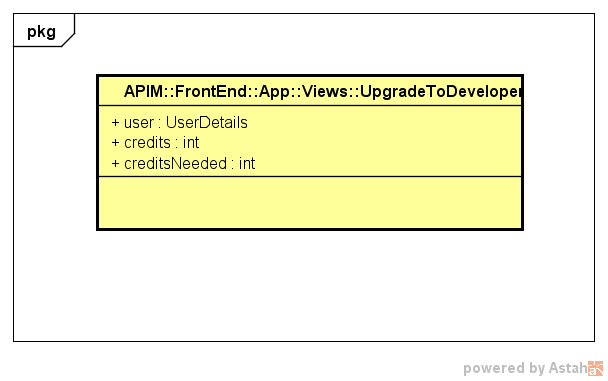
\includegraphics
	[width=0.7\linewidth]
	{images/APIM/FrontEnd/Views/UpgradeToDeveloper.png}
	\caption{APIM::FrontEnd::App::Views::UpgradeToDeveloper}
\end{figure}

\begin{itemize}
	\item \textbf{Descrizione:} View contenente il modulo per diventare sviluppatore all'interno dell'\progetto.
	\item \textbf{Attributi:}
	\begin{itemize}
		\item \textbf{user : UserDetails}\\
		Campo dati contenente le informazioni di un utente;
		\item \textbf{credits : int}\\
		Campo dati contenente i crediti personali di un utente;
		\item \textbf{creditsNeeded : int}\\
		Campo dati contenente i crediti necessari all'upgrade.
	\end{itemize}
	\item \textbf{Relazioni con altre classi:}
	\begin{itemize}
		\item Interagisce con il controller \textbf{UpgradeToDeveloperController};
	\end{itemize}
\end{itemize}

\paragraph{APIM::FrontEnd::App::Views::AdminAPIManager}

\begin{figure}[H]
	\centering
	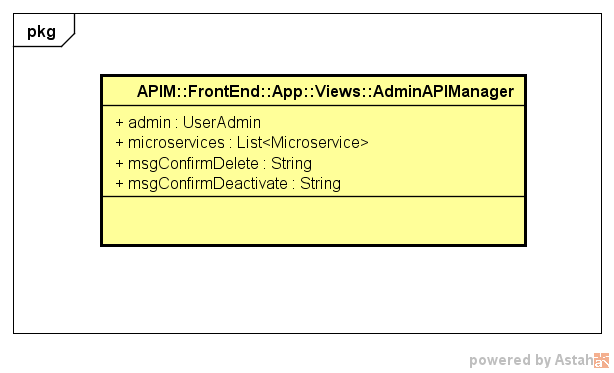
\includegraphics
	[width=0.7\linewidth]
	{images/APIM/FrontEnd/Views/AdminAPIManager.png}
	\caption{APIM::FrontEnd::App::Views::AdminAPIManager}
\end{figure}

\begin{itemize}
	\item \textbf{Descrizione:} View contenente le operazioni dell'amministratore sulle API dell'\progetto.
	\item \textbf{Attributi:}
	\begin{itemize}
		\item \textbf{admin : UserAdmin}\\
		Campo dati contenente le informazioni di un admin;
		\item \textbf{microservices : List<Microservice>}\\
		Campo dati contenente una lista di microservizi;
		\item \textbf{msgConfirmDelete : string}\\
		Campo dati contenente un messaggio di conferma eliminazione di un API.
		\item \textbf{msgConfirmDeactivate : string}\\
		Campo dati contenente un messaggio di conferma disattivazione di un API.
	\end{itemize}
	\item \textbf{Relazioni con altre classi:}
	\begin{itemize}
		\item Interagisce con il controller \textbf{AdminAPIManagerController};
		\item Il model \textbf{MicroserviceModel} contiene le informazioni per rappresentare un microservizio.
	\end{itemize}
\end{itemize}

\paragraph{APIM::FrontEnd::App::Views::AdminLogin}

\begin{figure}[H]
	\centering
	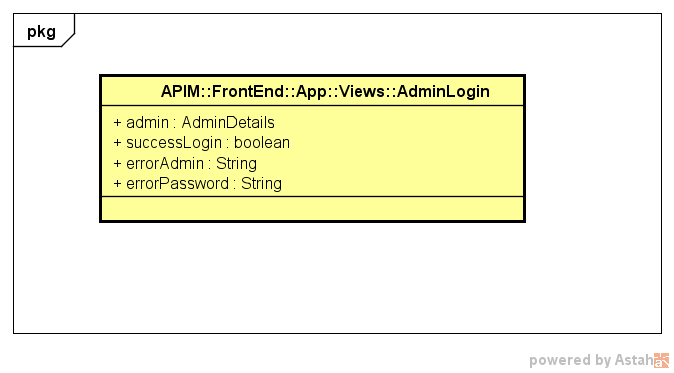
\includegraphics
	[width=0.7\linewidth]
	{images/APIM/FrontEnd/Views/AdminLogin.png}
	\caption{APIM::FrontEnd::App::Views::AdminLogin}
\end{figure}

\begin{itemize}
	\item \textbf{Descrizione:} View contenente il form necessario affinchè l'amministratore possa effettuare il login ed autenticarsi al sistema.\\
	\item \textbf{Attributi:}
	\begin{itemize}
		\item \textbf{admin : AdminDetails}\\
		Campo dati contenente le informazioni di un admin;
		\item \textbf{successLogin : boolean}\\
		Campo dati contenente il flag per il login di un amministratore;
		\item \textbf{errorAdmin : string}\\
		Campo dati contenente un messaggio di errore di autenticazione dell'admin;
		\item \textbf{errorPassword : string}\\
		Campo dati contenente un messaggio di errore password errata.
	\end{itemize}
	\item \textbf{Relazioni con altre classi:}
	\begin{itemize}
		\item Interagisce con il controller \textbf{AdminLoginController};
	\end{itemize}
\end{itemize}

\paragraph{APIM::FrontEnd::App::Views::Logout}

\begin{figure}[H]
	\centering
	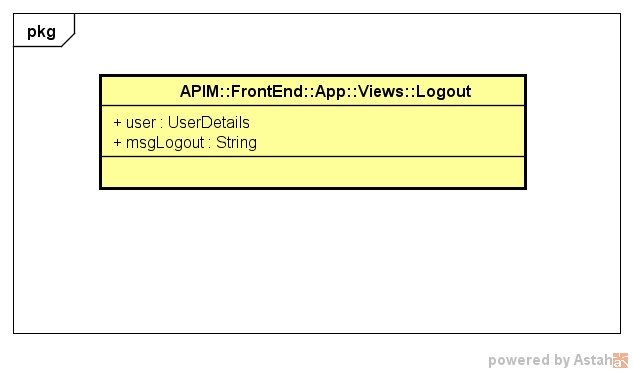
\includegraphics
	[width=0.7\linewidth]
	{images/APIM/FrontEnd/Views/Logout.png}
	\caption{APIM::FrontEnd::App::Views::Logout}
\end{figure}

\begin{itemize}
	\item \textbf{Descrizione:} View contenente la conferma di logout dall'\progetto.
	\item \textbf{Attributi:}
	\begin{itemize}
		\item \textbf{user : UserDetails}\\
		Campo dati contenente le informazioni di un utente;
		\item \textbf{msgLogout : string}\\
		Campo dati contenente un messaggio di avvenuto logout dalla piattaforma;
	\end{itemize}
	\item \textbf{Relazioni con altre classi:}
	\begin{itemize}
		\item Interagisce con il controller \textbf{LogoutController};
	\end{itemize}
\end{itemize}

\paragraph{APIM::FrontEnd::App::Views::UpdateInfoAPI}

\begin{figure}[H]
	\centering
	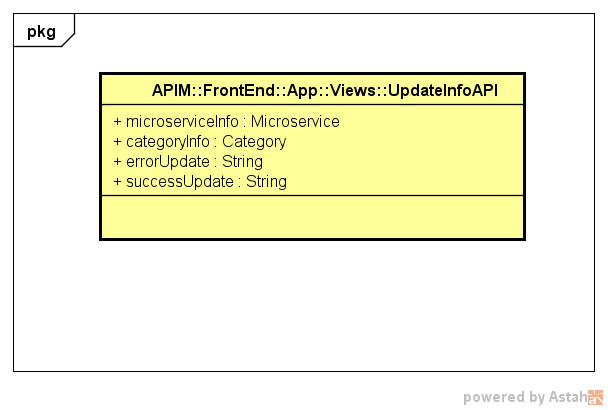
\includegraphics
	[width=0.7\linewidth]
	{images/APIM/FrontEnd/Views/UpdateInfoAPI.png}
	\caption{APIM::FrontEnd::App::Views::UpdateInfoAPI}
\end{figure}

\begin{itemize}
	\item \textbf{Descrizione:} View contenente il form dedicato modifica delle informazioni di una API presente nel marketplace \progetto.
	\item \textbf{Attributi:}
	\begin{itemize}
		\item \textbf{microserviceInfo : Microservice}\\
		Campo dati contenente le informazioni di un microservizio;
		\item \textbf{categoryInfo : category}\\
		Campo dati contenente le informazioni della categoria di un microservizio;
		\item \textbf{errorUpdate : string}\\
		Campo dati contenente un messaggio di errore di modifica delle informazioni API;
		\item \textbf{successUpdate : string}\\
		Campo dati contenente un messaggio di avvenuta modifica delle informazioni.
	\end{itemize}
	\item \textbf{Relazioni con altre classi:}
	\begin{itemize}
		\item Interagisce con il controller \textbf{UpdateInfoAPIController};
		\item Il model \textbf{MicroserviceModel} contiene le informazioni per rappresentare un microservizio.
	\end{itemize}
\end{itemize}

\paragraph{APIM::FrontEnd::App::Views::RechargeCredits}

\begin{figure}[H]
	\centering
	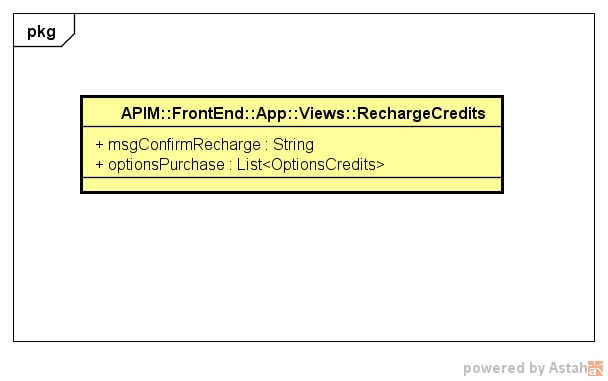
\includegraphics
	[width=0.7\linewidth]
	{images/APIM/FrontEnd/Views/RechargeCredits.png}
	\caption{APIM::FrontEnd::App::Views::RechargeCredits}
\end{figure}

\begin{itemize}
	\item \textbf{Descrizione:} View contenente la possibilità di scegliere quanti crediti ricaricare sul conto personale tra i tagli disponibili.
	\item \textbf{Attributi:}
	\begin{itemize}
		\item \textbf{msgConfirmRecharge : string}\\
		Campo dati contenente un messaggio di conferma della ricarica crediti;
		\item \textbf{optionsPurchase : List<OptionsCredits>}\\
		Campo dati contenente le opzioni di acquisto dei crediti previste.
	\end{itemize}
	\item \textbf{Relazioni con altre classi:}
	\begin{itemize}
		\item Interagisce con il controller \textbf{RechargeCreditsController}.
	\end{itemize}
\end{itemize}

\paragraph{APIM::FrontEnd::App::Views::ShowUserDetails}

\begin{figure}[H]
	\centering
	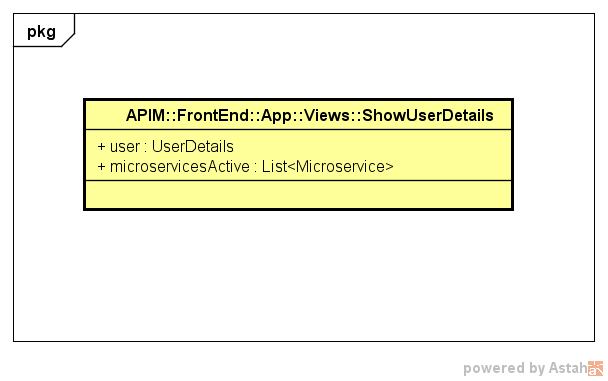
\includegraphics
	[width=0.7\linewidth]
	{images/APIM/FrontEnd/Views/ShowUserDetails.png}
	\caption{APIM::FrontEnd::App::Views::ShowUserDetails}
\end{figure}

\begin{itemize}
	\item \textbf{Descrizione:} View contenente le informazioni personali di un utente visualizzabili da altri fruitori del marketplace \progetto.
	\item \textbf{Attributi:}
	\begin{itemize}
		\item \textbf{user : UserDetails}\\
		Campo dati contenente i dati di utente;
		\item \textbf{microservicesActive : List<Microservice>}\\
		Campo dati contenente la lista dei microservizi attivi per il dato utente.
	\end{itemize}
	\item \textbf{Relazioni con altre classi:}
	\begin{itemize}
		\item Interagisce con il controller \textbf{ShowUserDetailsController};
		\item Il model \textbf{MicroserviceModel} contiene le informazioni per rappresentare un microservizio;
		\item Il model \textbf{UserDetailsModel} contiene le informazioni per rappresentare un utente.
	\end{itemize}
\end{itemize}

%Fine views

\subsection{APIM::FrontEnd::App::Models}

\subsubsection{Informazioni generali}

\begin{figure}[H]
	\centering
	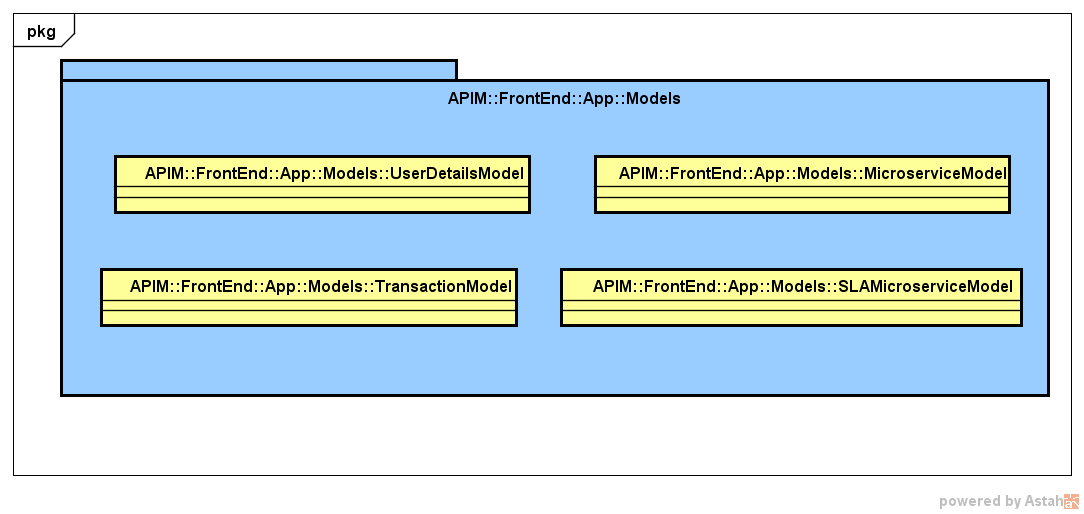
\includegraphics
	[width=0.7\linewidth]
	{images/APIM/FrontEnd/Models/Models.png}
	\caption{APIM::FrontEnd:App:Models}
\end{figure}

\begin{itemize}
	\item \textbf{Descrizione:} Il package Models contiene le classi che definiscono le strutture dei dati di utenti, microservizi, transazioni e sondaggi SLA.
	\item \textbf{Relazioni con altre classi:}
		\begin{itemize}
			\item Interagisce con i package \textbf{Controllers} e \textbf{Views} per garantire il dynamic binding di AngularJS.
		\end{itemize}
\end{itemize}

\subsubsection{Classi}

\paragraph{APIM::FrontEnd::App::Models::UserDetailsModel}

\begin{figure}[H]
	\centering
	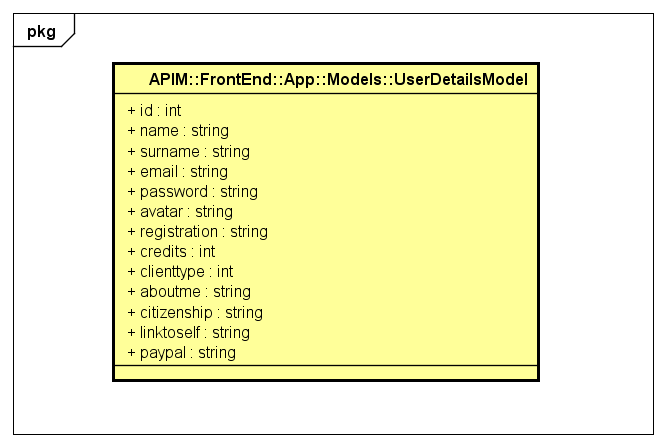
\includegraphics
	[width=0.7\linewidth]
	{images/APIM/FrontEnd/Models/UserDetailsModel.png}
	\caption{APIM::FrontEnd::App::Models:UserDetailsModel}
\end{figure}

\begin{itemize}
	\item \textbf{Descrizione:} UserDetailsModel che rappresenta un utente e che contiene tutte le informazioni
necessarie alla presentazione del contenuto di un utente, sia nella visualizzazione che nella gestione di un profilo.
	\item \textbf{Attributi:}
		\begin{itemize}
			\item \textbf{id : int}\\
			Id dell'utente;
			\item \textbf{name : string}\\
			Nome dell'utente;
			\item \textbf{surname : string}\\
			Cognome dell'utente;
			\item \textbf{email : string}\\
			Email dell'utente;
			\item \textbf{password : string}\\
			Password dell'utente;
			\item \textbf{avatar : string}\\
			Avatar dell'utente;
			\item \textbf{registration : string}\\
			Data di registrazione dell'utente;
			\item \textbf{credits : int}\\
			Crediti dell'utente;
			\item \textbf{clientType : int}\\
			Tipo di account dell'utente;
			\item \textbf{aboutMe : string}\\
			AboutMe dell'utente sviluppatore;
			\item \textbf{citizenship : string}\\
			Cittadinanza dell'utente sviluppatore;
			\item \textbf{linkToSelf : string}\\
			Link al sito esterno dell'utente sviluppatore;
			\item \textbf{paypal : string}\\
			Email paypal dell'utente sviluppatore.
		\end{itemize}
	\item \textbf{Relazioni con altre classi:}
		\begin{itemize}
			\item Interagisce con il controller \textbf{LoginController};
			\item Interagisce con il controller \textbf{APIController};
			\item Interagisce con il controller \textbf{ProfileManagerController};
			\item Interagisce con il controller \textbf{ResetPasswordController};
			\item Interagisce con il controller \textbf{PasswordRecoveryController};
	\end{itemize}
\end{itemize}

\paragraph{APIM::FrontEnd::App::Models::TransactionModel}

\begin{figure}[H]
	\centering
	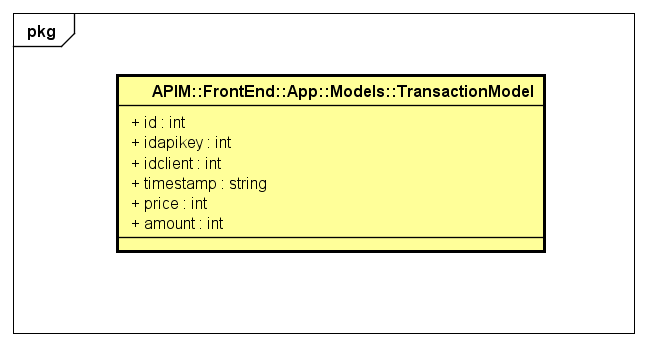
\includegraphics
	[width=0.7\linewidth]
	{images/APIM/FrontEnd/Models/TransactionModel.png}
	\caption{APIM::FrontEnd::App::Models::TransactionModel}
\end{figure}

\begin{itemize}
	\item \textbf{Descrizione:} TransactionModel rappresenta una transazione avvenuta e che contiene
tutte le informazioni necessarie alla presentazione del contenuto di una transazione,
sia nella visualizzazione che nella gestione.
	\item \textbf{Attributi:}
		\begin{itemize}
			\item \textbf{id : int}\\
			Id della transazione;
			\item \textbf{idAPIKey : int}\\
			Id dell'apikey;
			\item \textbf{idClient : int}\\
			Id del cliente;
			\item \textbf{timestamp : int}\\
			Data ed ora della transazione;
			\item \textbf{price : int}\\
			Prezzo della transazione;
			\item \textbf{amount : int}\\
			Ammontare quantitativo della transazione.
		\end{itemize}
	\item \textbf{Relazioni con altre classi:}
		\begin{itemize}
			\item Interagisce con il controller \textbf{TransactionsListController};
			\item Interagisce con il controller \textbf{APIPurchasedController}.
		\end{itemize}
\end{itemize}

\paragraph{APIM::FrontEnd::App::Models::MicroserviceModel}

\begin{figure}[H]
	\centering
	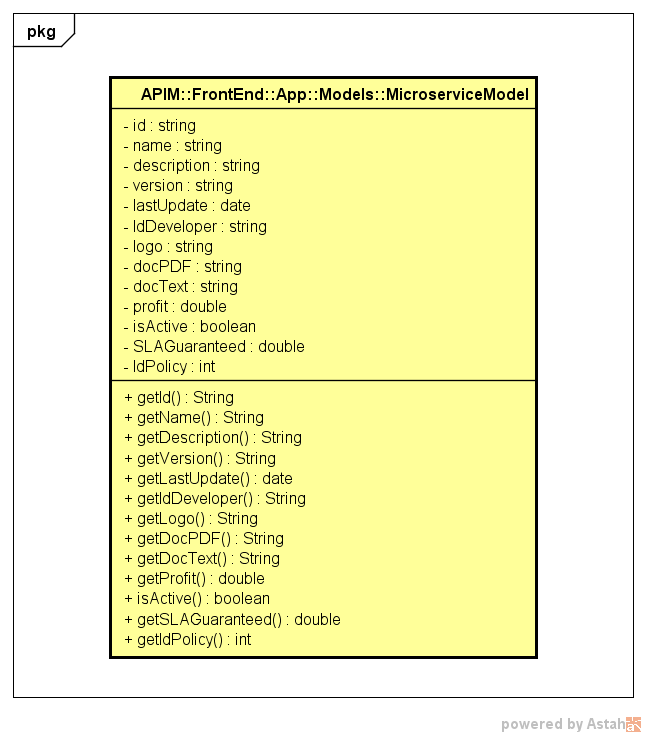
\includegraphics
	[width=0.7\linewidth]
	{images/APIM/FrontEnd/Models/MicroserviceModel.png}
	\caption{APIMarket::FrontEnd::App::Models::MicroserviceModel}
\end{figure}

\begin{itemize}
	\item \textbf{Descrizione:} MicroserviceModel rappresenta un microservizio e che contiene tutte le
informazioni necessarie alla presentazione del contenuto di un microservizio, sia nella visualizzazione che nella gestione.
	\item \textbf{Attributi:}
		\begin{itemize}
			\item \textbf{id : int}\\
			Id del microservizio;
			\item \textbf{name : string}\\
			Nome del microservizio;
			\item \textbf{description : string}\\
			Descrizione del microservizio;
			\item \textbf{version : string}\\
			Versione corrente del microservizio;
			\item \textbf{lastUpdate : string}\\
			Data ultimo aggiornamento del microservizio;
			\item \textbf{idDeveloper : string}\\
			Id dello sviluppatore del microservizio;
			\item \textbf{logo : string}\\
			Link al logo del microservizio;
			\item \textbf{docPDF : string}\\
			Link al file PDF del microservizio;
			\item \textbf{docExt : string}\\
			Link alla documentazione esterna del microservizio;
			\item \textbf{profit : int}\\
			Percentuale profitto dello sviluppatore del microservizio;
			\item \textbf{isActive : bool}\\
			Funzionamento attuale del microservizio;
			\item \textbf{SLAGuaranteed : double}\\
			SLA garantita dal microservizio;
			\item \textbf{idPolicy : int}\\
			Id della policy di vendita del microservizio.
		\end{itemize}
	\item \textbf{Relazioni con altre classi:}
		\begin{itemize}
			\item Interagisce con il controller \textbf{APIRegisteredController};
			\item Interagisce con il controller \textbf{RegisterAPIController}.	
			\item Interagisce con il controller \textbf{PolicyCallController};
			\item Interagisce con il controller \textbf{PolicyTimeController};
			\item Interagisce con il controller \textbf{PolicyTrafficController};
			\item Interagisce con il controller \textbf{APIPurchasedController};
			\item Interagisce con il controller \textbf{APIListController}.
		\end{itemize}
\end{itemize}

\paragraph{APIM::FrontEnd::App::Models::SLAMicroserviceModel}

\begin{figure}[H]
	\centering
	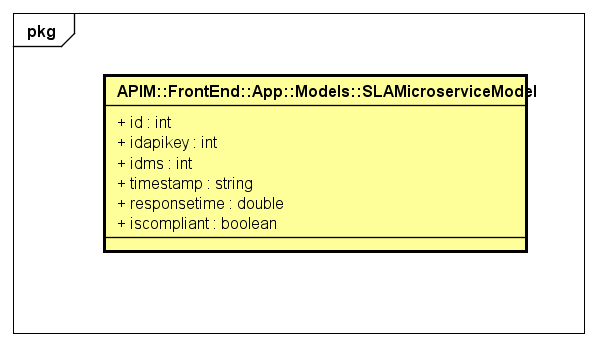
\includegraphics
	[width=0.7\linewidth]
	{images/APIM/FrontEnd/Models/SLAMicroserviceModel.png}
	\caption{APIM::FrontEnd::App::Models::SLAMicroserviceModel}
\end{figure}

\begin{itemize}
	\item \textbf{Descrizione:} SLAMicroserviceModel rappresenta la SLA di un microservizio e che
contiene tutte le informazioni necessarie alla presentazione del contenuto di SLA di un microservizio, sia nella visualizzazione che nella gestione.
	\item \textbf{Attributi:}
		\begin{itemize}
			\item \textbf{id : int}\\
			Id del sondaggio SLA;
			\item \textbf{idapikey : int}\\
			Id dell'apike attribuita al sondaggio SLA;
			\item \textbf{idMS : int}\\
			Id del microservizio attribuito al sondaggio SLA;
			\item \textbf{timestamp : string}\\
			Data ed ora del sondaggio SLA;
			\item \textbf{responseTime : int}\\
			Tempo di risposta del sondaggio SLA;
			\item \textbf{isCompliant : boolean}\\
			Indicatore del rispetto del sondaggio SLA.
		\end{itemize}
	\item \textbf{Relazioni con altre classi:}
		\begin{itemize}
			\item Interagisce con il controller \textbf{PolicyCallController};
			\item Interagisce con il controller \textbf{PolicyTimeController};
			\item Interagisce con il controller \textbf{PolicyTrafficController};
			\item Interagisce con il controller \textbf{RegisterAPIController}.		
		\end{itemize}
\end{itemize}

%Fine models

\subsection{APIM::FrontEnd::App::Controllers}

\subsubsection{Informazioni generali}

\begin{figure}[H]
	\centering
	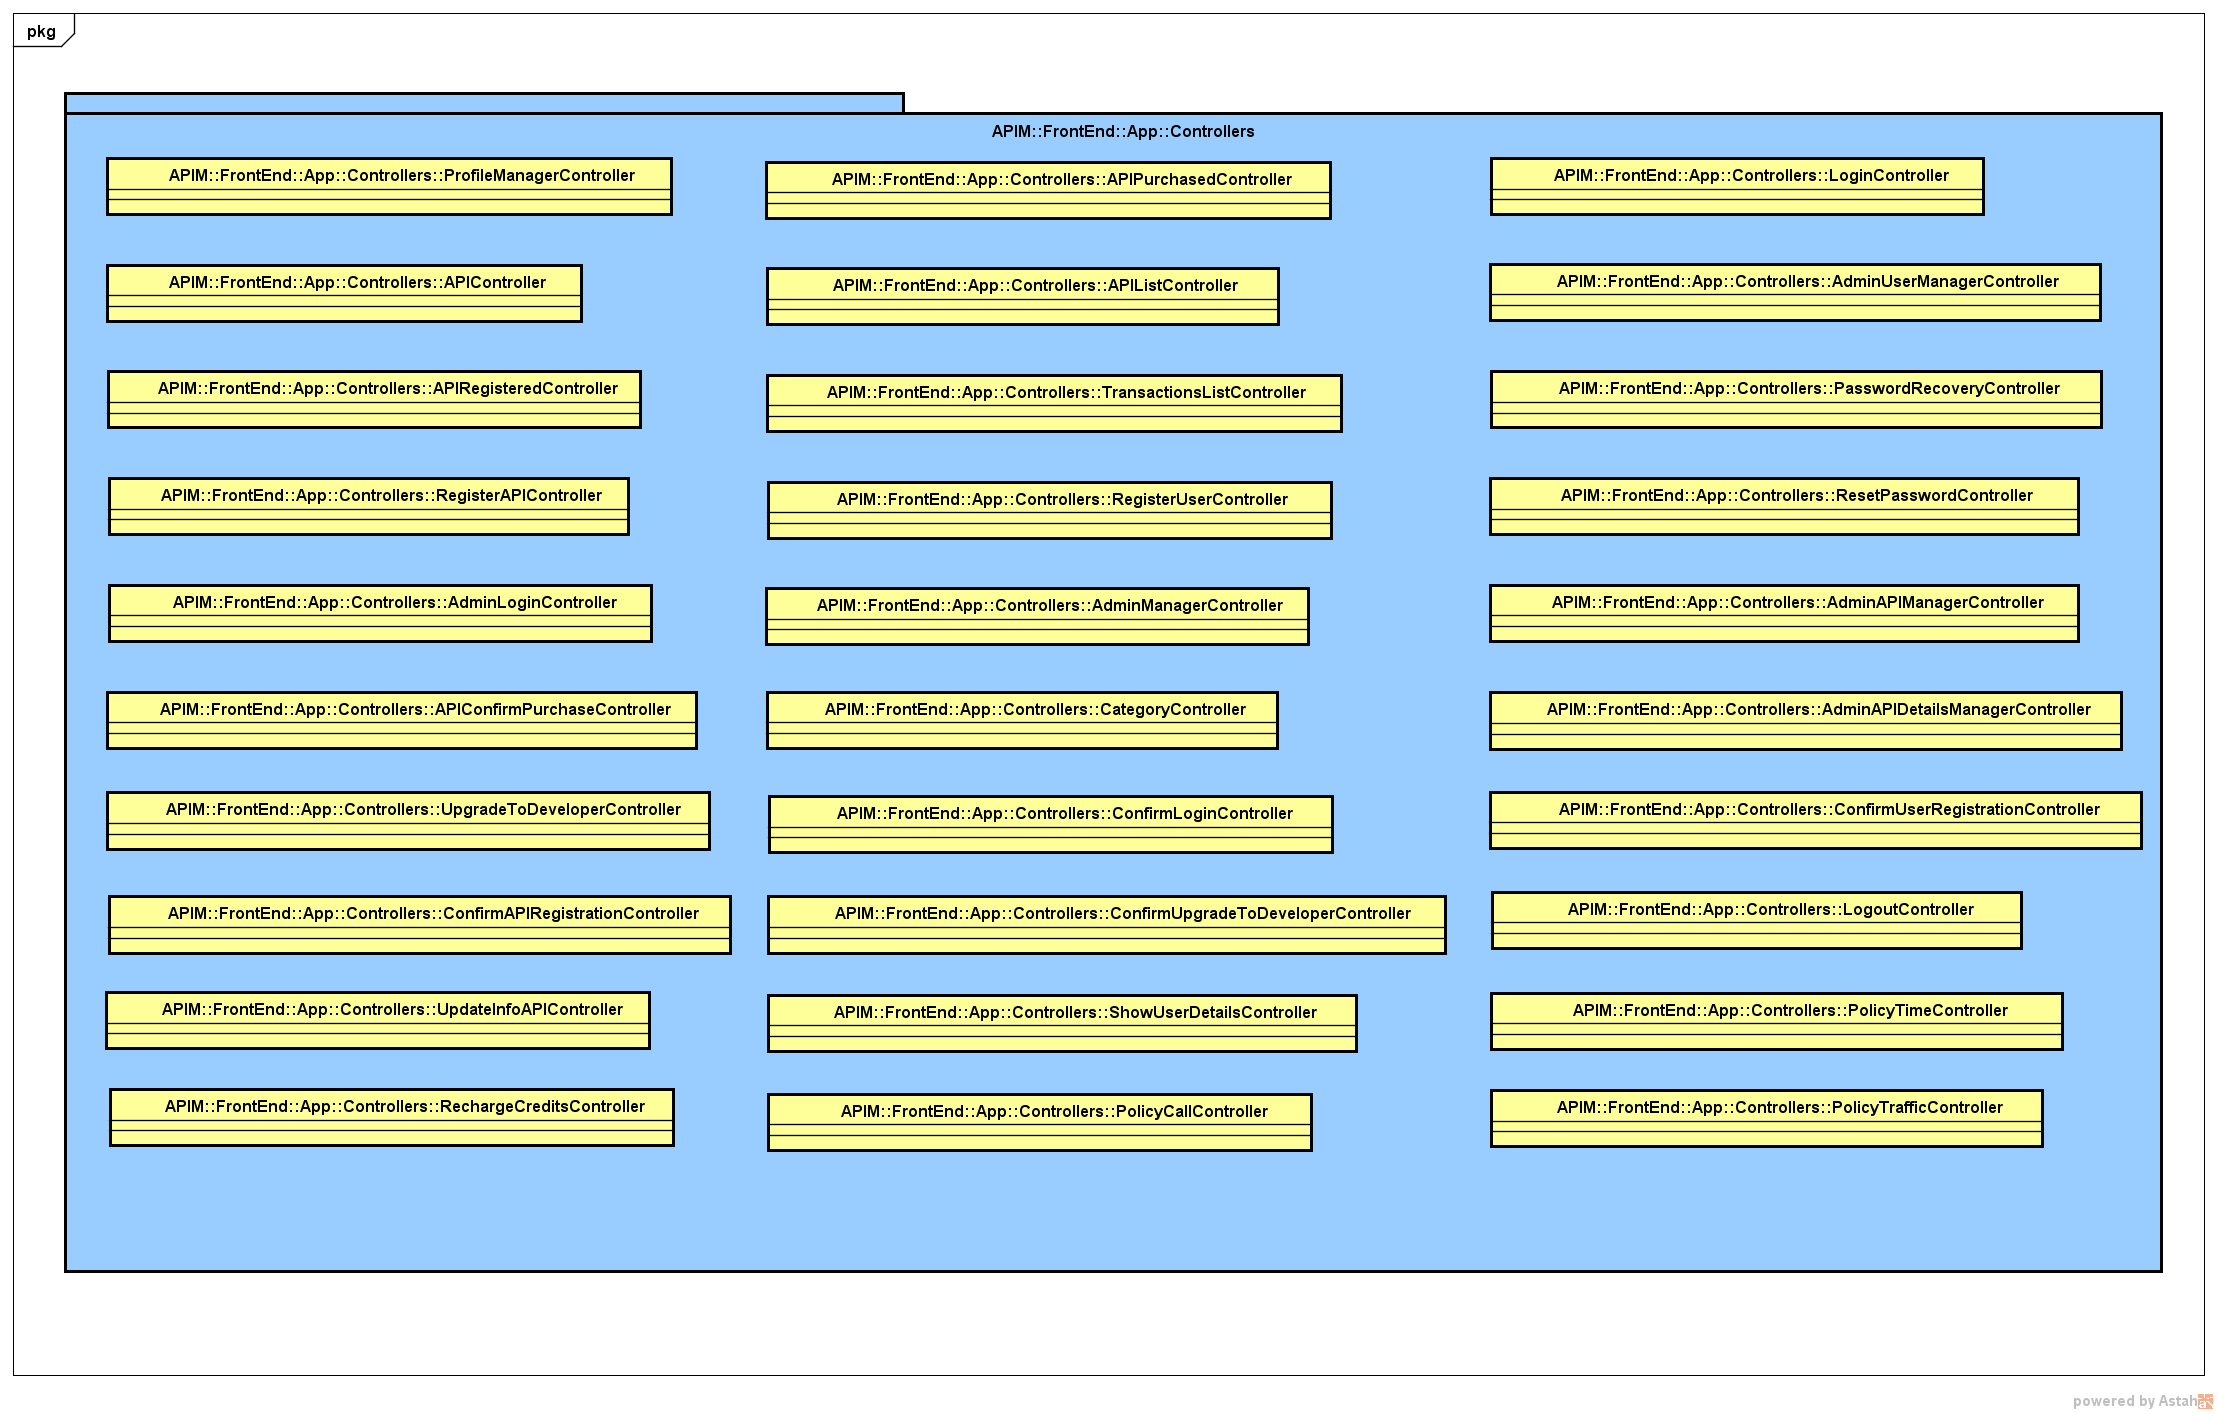
\includegraphics
	[width=0.7\linewidth]
	{images/APIM/FrontEnd/Controllers/Controllers.png}
	\caption{APIM::FrontEnd::App::Controllers}
\end{figure}

\begin{itemize}
	\item \textbf{Descrizione:} Il package Controllers contiene tutti i controller dell'applicazione.
	\item \textbf{Relazioni con altre classi:}
		\begin{itemize}
			\item Il package \textbf{View} è collegato ad un controller per gestirne la visualizzazione delle pagine ed il routing; 
			\item Il package \textbf{Models} contiene le strutture dati cui i controllers si riferiscono.
		\end{itemize}
\end{itemize}

\subsubsection{Classi}

\paragraph{APIM::FrontEnd::App::Controllers::AdminAPIDetailsManagerController}

\begin{figure}[H]
	\centering
	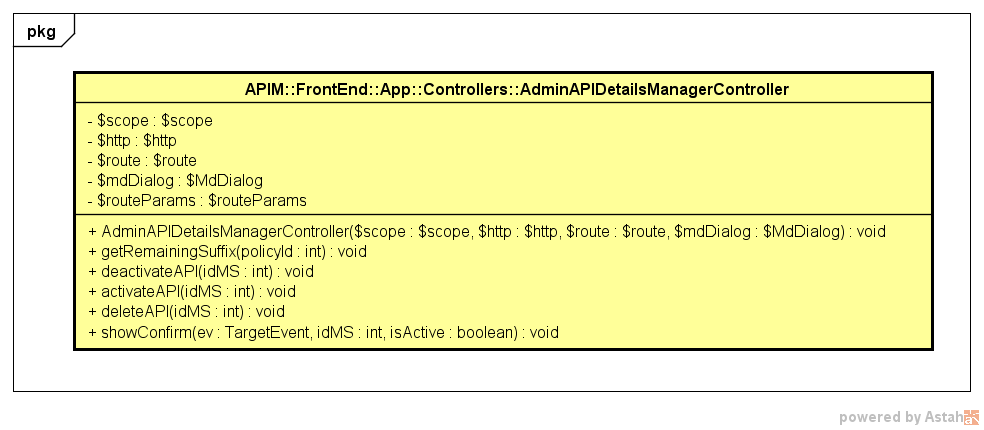
\includegraphics
	[width=0.7\linewidth]
	{images/APIM/FrontEnd/Controllers/AdminAPIDetailsManagerController.png}
	\caption{APIM::FrontEnd::App::Controllers::AdminAPIDetailsManagerController}
\end{figure}

\begin{itemize}
	\item \textbf{Descrizione:} classe che permette di visualizzare le statistiche di un'API, attivarla, disattivarla o eliminarla.
	\item \textbf{Attributi:}
	\begin{itemize}
		\item \textbf{\$scope : \$scope}\\
		Campo dati contenente un riferimento all'oggetto \$scope creato da AngularJS, viene utilizzato come mezzo di comunicazione tra il controller e la view. Contiene gli oggetti che definiscono il model dell'applicazione;
		
		\item \textbf{\$http : \$http }\\
		Campo dati che contiene un riferimento al servizio \$http che permette la comunicazione con il protocollo HTTP;
		
		\item \textbf{\$route : \$route }\\
		Campo dati contenente il riferimento all'oggetto globale \$route creato da AngularJS. Viene utilizzato per le funzioni di routing;
		
		\item \textbf{\$mdDialog : \$mdDialog }\\
		Campo dati contenente il riferimento all'oggetto globale \$mdDialog creato da AngularJS. Viene utilizzato per creare finestre di popup;
		
		\item \textbf{\$routeParams : \$routeParams }\\
		Campo dati contenente il riferimento all'oggetto globale \$routeParams creato da AngularJS. Viene utilizzato per riferirsi alle variabili GET e POST;
		
		
	\end{itemize}
	\item \textbf{Metodi:}
	\begin{itemize}
		
		\item \textbf{AdminAPIDetailsManagerController(\$scope : \$scope, \$http : \$http, \$route : \$route, \$mdDialog : \$mdDialog, \$routeParams : \$routeParams)}\\
		Metodo costruttore della classe.
		\begin{description}
			\item[\textbf{Parametri:}]
		\end{description}
		\begin{itemize}
			\item \textbf{\$scope : \$scope}\\
			Parametro che contiene un riferimento all'oggetto \$scope di AngularJS, impiegato nella comunicazione tra i rispettivi view e controller. Contiene gli oggetti che definiscono i model dell'applicazione;
			
			\item \textbf{\$http : \$http}\\
			Parametro che contiene il riferimento all'oggetto globale \$http di AngularJS. Viene utilizzato per la comunicazione con il protocollo HTTP.
			
			\item \textbf{\$route : \$route}\\
			Parametro che contiene il riferimento all'oggetto globale \$route di AngularJS. Viene utilizzato per le funzioni di routing.
			
			\item \textbf{\$mdDialog : \$mdDialog}\\
			Parametro che contiene il riferimento all'oggetto globale \$mdDialog di AngularJS. Viene utilizzato per creare finestre di popup.
			
			\item \textbf{\$routeParams : \$routeParams}\\
			Parametro che contiene il riferimento all'oggetto globale \$routeParams di AngularJS. Viene utilizzato per riferirsi alle variabili GET e POST.
			
		\end{itemize}
		
		\item \textbf{getRemainingSuffix(policyId : int) : void}\\
		Metodo per identificare la tipologia di policy dell'API. Si serve di un'operazione di un servizio esposto dal package \textbf{Services}.
		\begin{description}
			\item[\textbf{Parametri:}]
		\end{description}
		\begin{itemize}
			\item \textbf{policyId : int}\\
			Identificativo del tipo di policy;
		\end{itemize}
		
		\item \textbf{deactivateAPI(IdMS : int) : void}\\
		Metodo per disattivare l'API. Si serve di un'operazione di un servizio esposto dal package \textbf{Services}.
		\begin{description}
			\item[\textbf{Parametri:}]
		\end{description}
		\begin{itemize}
			\item \textbf{IdMS : int}\\
			Identificativo dell'API;
		\end{itemize}
		
		\item \textbf{activateAPI(IdMS : int) : void}\\
		Metodo per attivare l'API. Si serve di un'operazione di un servizio esposto dal package \textbf{Services}.
		\begin{description}
			\item[\textbf{Parametri:}]
		\end{description}
		\begin{itemize}
			\item \textbf{IdMS : int}\\
			Identificativo dell'API;
		\end{itemize}
		
		\item \textbf{deleteAPI(IdMS : int) : void}\\
		Metodo per eliminare l'API. Si serve di un'operazione di un servizio esposto dal package \textbf{Services}.
		\begin{description}
			\item[\textbf{Parametri:}]
		\end{description}
		\begin{itemize}
			\item \textbf{IdMS : int}\\
			Identificativo dell'API;
		\end{itemize}
		
		\item \textbf{showConfirm(ev : TargetEvent, IdMS : int, isActive : boolean) : void}\\
		Metodo per mostrare una finestra di conferma di elimninazione dell'API. Si serve di un'operazione di un servizio esposto dal package \textbf{Services}.
		\begin{description}
			\item[\textbf{Parametri:}]
		\end{description}
		\begin{itemize}
			\item \textbf{ev : TargetEvent}\\
			Identifica il target che ha fatto scatenare l'evento di apertura del popup;
			
			\item \textbf{IdMS : int}\\
			Identificativo dell'API;
			
			\item \textbf{boolean : isActive}\\
			Identifica lo stato dell'API;
			
		\end{itemize}
		
	\end{itemize}
	\item \textbf{Relazioni con altre classi:}
	\begin{itemize}
		\item Ricava i dati necessari dal package \textbf{Services};
		\item Gestisce il funzionamento della view \textbf{AdminAPIDetails};
	\end{itemize}
\end{itemize}

\paragraph{APIM::FrontEnd::App::Controllers::AdminAPIManagerController}

\begin{figure}[H]
	\centering
	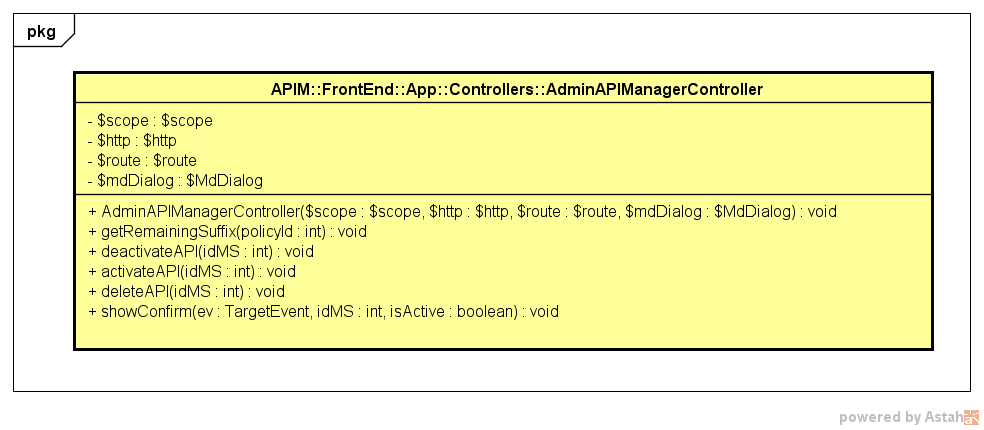
\includegraphics
	[width=0.7\linewidth]
	{images/APIM/FrontEnd/Controllers/AdminAPIManagerController.png}
	\caption{APIM::FrontEnd::App::Controllers::AdminAPIManagerController}
\end{figure}

\begin{itemize}
	\item \textbf{Descrizione:} classe che permette di fornire la lista di tutte le API presenti e di effettuare alcune operazioni come attivazione, disattivazione ed eliminazione.
	\item \textbf{Attributi:}
	\begin{itemize}
		
		\item \textbf{\$scope : \$scope}\\
		Campo dati contenente un riferimento all'oggetto \$scope creato da AngularJS, viene utilizzato come mezzo di comunicazione tra il controller e la view. Contiene gli oggetti che definiscono il model dell'applicazione;
		
		\item \textbf{\$http : \$http }\\
		Campo dati che contiene un riferimento al servizio \$http che permette la comunicazione con il protocollo HTTP;
		
		\item \textbf{\$route : \$route }\\
		Campo dati contenente il riferimento all'oggetto globale \$route creato da AngularJS. Viene utilizzato per le funzioni di routing;
		
		\item \textbf{\$mdDialog : \$mdDialog }\\
		Campo dati contenente il riferimento all'oggetto globale \$mdDialog creato da AngularJS. Viene utilizzato per creare finestre di popup;
		
		\item \textbf{\$routeParams : \$routeParams }\\
		Campo dati contenente il riferimento all'oggetto globale \$routeParams creato da AngularJS. Viene utilizzato per riferirsi alle variabili GET e POST;
		
		
	\end{itemize}
	\item \textbf{Metodi:}
	\begin{itemize}
		
		\item \textbf{AdminAPIManagerController(\$scope : \$scope, \$http : \$http, \$route : \$route, \$mdDialog : \$mdDialog, \$routeParams : \$routeParams)}\\
		Metodo costruttore della classe;
		\begin{description}
			\item[\textbf{Parametri:}]
		\end{description}
		\begin{itemize}
			\item \textbf{\$scope : \$scope}\\
			Parametro che contiene un riferimento all'oggetto \$scope di AngularJS, impiegato nella comunicazione tra i rispettivi view e controller. Contiene gli oggetti che definiscono i model dell'applicazione;
			
			\item \textbf{\$http : \$http}\\
			Parametro che contiene il riferimento all'oggetto globale \$http di AngularJS. Viene utilizzato per la comunicazione con il protocollo HTTP.
			
			\item \textbf{\$route : \$route}\\
			Parametro che contiene il riferimento all'oggetto globale \$route di AngularJS. Viene utilizzato per le funzioni di routing.
			
			\item \textbf{\$mdDialog : \$mdDialog}\\
			Parametro che contiene il riferimento all'oggetto globale \$mdDialog di AngularJS. Viene utilizzato per creare finestre di popup.
			
			\item \textbf{\$routeParams : \$routeParams}\\
			Parametro che contiene il riferimento all'oggetto globale \$routeParams di AngularJS. Viene utilizzato per riferirsi alle variabili GET e POST.
			
		\end{itemize}
		
		\item \textbf{getRemainingSuffix(policyId : int) : void}\\
		Metodo per identificare la tipologia di policy dell'API. Si serve di un'operazione di un servizio esposto dal package \textbf{Services}.
		\begin{description}
			\item[\textbf{Parametri:}]
		\end{description}
		\begin{itemize}
			\item \textbf{policyId : int}\\
			Identificativo del tipo di policy;
		\end{itemize}
		
		\item \textbf{deactivateAPI(IdMS : int) : void}\\
		Metodo per disattivare l'API. Si serve di un'operazione di un servizio esposto dal package \textbf{Services}.
		\begin{description}
			\item[\textbf{Parametri:}]
		\end{description}
		\begin{itemize}
			\item \textbf{IdMS : int}\\
			Identificativo dell'API;
		\end{itemize}
		
		\item \textbf{activateAPI(IdMS : int) : void}\\
		Metodo per attivare l'API. Si serve di un'operazione di un servizio esposto dal package \textbf{Services}.
		\begin{description}
			\item[\textbf{Parametri:}]
		\end{description}
		\begin{itemize}
			\item \textbf{IdMS : int}\\
			Identificativo dell'API;
		\end{itemize}
		
		\item \textbf{deleteAPI(IdMS : int) : void}\\
		Metodo per eliminare l'API. Si serve di un'operazione di un servizio esposto dal package \textbf{Services}.
		\begin{description}
			\item[\textbf{Parametri:}]
		\end{description}
		\begin{itemize}
			\item \textbf{IdMS : int}\\
			Identificativo dell'API;
		\end{itemize}
		
		\item \textbf{showConfirm(ev : TargetEvent, IdMS : int, isActive : boolean) : void}\\
		Metodo per mostrare una finestra di conferma di elimninazione dell'API. Si serve di un'operazione di un servizio esposto dal package \textbf{Services}.
		\begin{description}
			\item[\textbf{Parametri:}]
		\end{description}
		\begin{itemize}
			\item \textbf{ev : TargetEvent}\\
			Identifica il target che ha fatto scatenare l'evento di apertura del popup;
			
			\item \textbf{IdMS : int}\\
			Identificativo dell'API;
			
			\item \textbf{boolean : isActive}\\
			Identifica lo stato dell'API;
			
		\end{itemize}
		
		
	\end{itemize}
	\item \textbf{Relazioni con altre classi:}
	\begin{itemize}
		\item Ricava i dati necessari dal package \textbf{Services};
		\item Gestisce il funzionamento della view \textbf{AdminAPIDetails};
	\end{itemize}
\end{itemize}

\paragraph{APIM::FrontEnd::App::Controllers::AdminLoginController}

\begin{figure}[H]
	\centering
	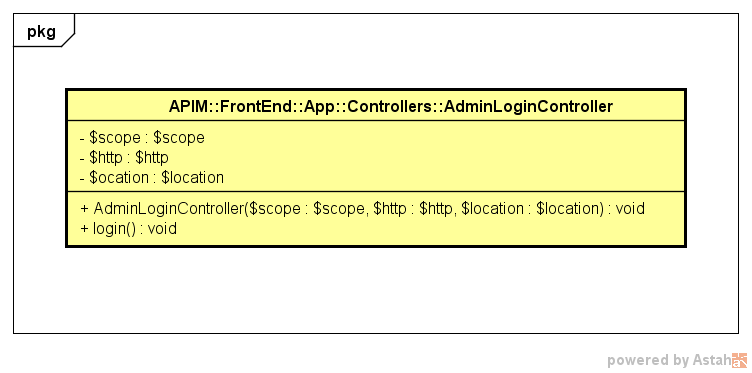
\includegraphics
	[width=0.7\linewidth]
	{images/APIM/FrontEnd/Controllers/AdminLoginController.png}
	\caption{APIM::FrontEnd::App::Controllers::AdminLoginController}
\end{figure}

\begin{itemize}
	\item \textbf{Descrizione:} AdminLoginController permette di effettuare il login all'area di amministrazione.
	\item \textbf{Attributi:}
	\begin{itemize}
		
		\item \textbf{\$scope : \$scope}\\
		Campo dati contenente un riferimento all'oggetto \$scope creato da AngularJS, viene utilizzato come mezzo di comunicazione tra il controller e la view. Contiene gli oggetti che definiscono il model dell'applicazione;
		
		\item \textbf{\$http : \$http }\\
		Campo dati che contiene un riferimento al servizio \$http che permette la comunicazione con il protocollo HTTP;
		
		\item \textbf{\$location : \$location }\\
		Campo dati contenente il riferimento all'oggetto globale \$location creato da AngularJS. Viene utilizzato per le funzioni di routing;
		
		
	\end{itemize}
	\item \textbf{Metodi:}
	\begin{itemize}
		
		\item \textbf{AdminLoginController(\$scope : \$scope, \$http : \$http, \$location : \$location)}\\
		Metodo costruttore della classe;
		\begin{description}
			\item[\textbf{Parametri:}]
		\end{description}
		\begin{itemize}
			\item \textbf{\$scope : \$scope}\\
			Parametro che contiene un riferimento all'oggetto \$scope di AngularJS, impiegato nella comunicazione tra i rispettivi view e controller. Contiene gli oggetti che definiscono i model dell'applicazione;
			
			\item \textbf{\$http : \$http}\\
			Parametro che contiene il riferimento all'oggetto globale \$http di AngularJS. Viene utilizzato per la comunicazione con il protocollo HTTP.
			
			\item \textbf{\$location : \$location}\\
			Parametro che contiene il riferimento all'oggetto globale \$location di AngularJS. Viene utilizzato per le funzioni di routing.
			
		\end{itemize}
		
		\item \textbf{login() : void}\\
		Metodo per effettuare il login. Si serve di un'operazione di un servizio esposto dal package \textbf{Services}.
		\begin{description}
			\item[\textbf{Parametri:}]
		\end{description}
		\begin{itemize}
			\item \textbf{void}\\
		\end{itemize}
		
	\end{itemize}
	\item \textbf{Relazioni con altre classi:}
	\begin{itemize}
		\item Ricava i dati necessari dal package \textbf{Services};
		\item Gestisce il funzionamento della view \textbf{AdminLogin};
	\end{itemize}
\end{itemize}


\paragraph{APIM::FrontEnd::App::Controllers::AdminUserManagerController}

\begin{figure}[H]
	\centering
	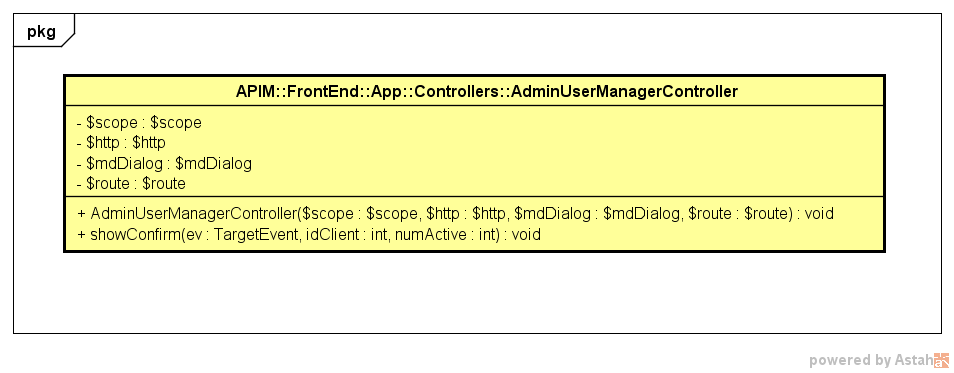
\includegraphics
	[width=0.7\linewidth]
	{images/APIM/FrontEnd/Controllers/AdminUserManagerController.png}
	\caption{APIM::FrontEnd::App::Controllers::AdminUserManagerController}
\end{figure}

\begin{itemize}
	\item \textbf{Descrizione:} classe che permette di gestire/moderare un utente (sostanzialmente eliminarlo).
	\item \textbf{Attributi:}
	\begin{itemize}
		
		\item \textbf{\$scope : \$scope}\\
		Campo dati contenente un riferimento all'oggetto \$scope creato da AngularJS, viene utilizzato come mezzo di comunicazione tra il controller e la view. Contiene gli oggetti che definiscono il model dell'applicazione;
		
		\item \textbf{\$http : \$http }\\
		Campo dati che contiene un riferimento al servizio \$http che permette la comunicazione con il protocollo HTTP;
		
		\item \textbf{\$route : \$route }\\
		Campo dati contenente il riferimento all'oggetto globale \$route creato da AngularJS. Viene utilizzato per le funzioni di routing;
		
		\item \textbf{\$mdDialog : \$mdDialog }\\
		Campo dati contenente il riferimento all'oggetto globale \$mdDialog creato da AngularJS. Viene utilizzato per creare finestre di popup;
		
		
	\end{itemize}
	\item \textbf{Metodi:}
	\begin{itemize}
		
		\item \textbf{AdminUserManagerController(\$scope : \$scope, \$http : \$http, \$route : \$route, \$mdDialog : \$mdDialog)}\\
		Metodo costruttore della classe;
		\begin{description}
			\item[\textbf{Parametri:}]
		\end{description}
		\begin{itemize}
			\item \textbf{\$scope : \$scope}\\
			Parametro che contiene un riferimento all'oggetto \$scope di AngularJS, impiegato nella comunicazione tra i rispettivi view e controller. Contiene gli oggetti che definiscono i model dell'applicazione;
			
			\item \textbf{\$http : \$http}\\
			Parametro che contiene il riferimento all'oggetto globale \$http di AngularJS. Viene utilizzato per la comunicazione con il protocollo HTTP.
			
			\item \textbf{\$route : \$route}\\
			Parametro che contiene il riferimento all'oggetto globale \$route di AngularJS. Viene utilizzato per le funzioni di routing.
			
			\item \textbf{\$mdDialog : \$mdDialog}\\
			Parametro che contiene il riferimento all'oggetto globale \$mdDialog di AngularJS. Viene utilizzato per creare finestre di popup.
			
		\end{itemize}
		
		
		\item \textbf{showConfirm(ev : TargetEvent, IdClient : int, isActivate : boolean) : void}\\
		Metodo per mostrare una finestra di conferma di elimninazione dell'utente. Si serve di un'operazione di un servizio esposto dal package \textbf{Services}.
		\begin{description}
			\item[\textbf{Parametri:}]
		\end{description}
		\begin{itemize}
			\item \textbf{ev : TargetEvent}\\
			Identifica il target che ha fatto scatenare l'evento di apertura del popup;
			
			\item \textbf{idClient : int}\\
			Identificativo dell'utente;
			
			\item \textbf{numActive : int}\\
			Numero di API attive per quel utente;
			
		\end{itemize}
		
	\end{itemize}
	\item \textbf{Relazioni con altre classi:}
	\begin{itemize}
		\item Ricava i dati necessari dal package \textbf{Services};
		\item Gestisce il funzionamento della view \textbf{AdminUserManager};
	\end{itemize}
\end{itemize}

\paragraph{APIM::FrontEnd::App::Controllers::APIConfirmPurchaseController}

\begin{figure}[H]
	\centering
	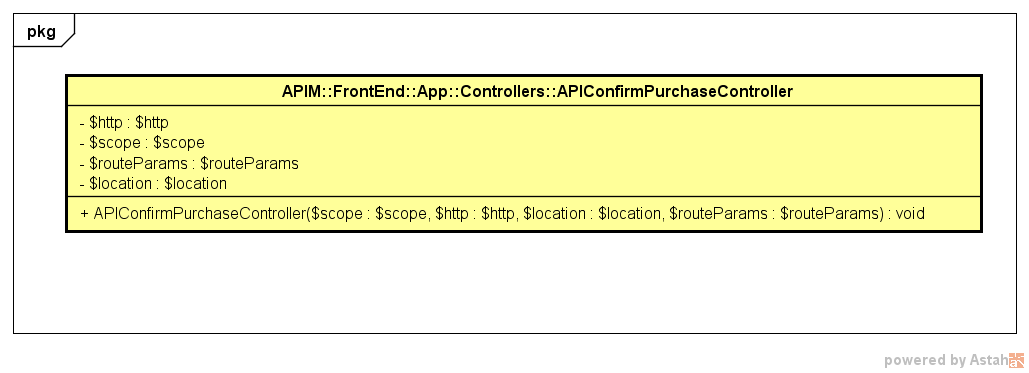
\includegraphics
	[width=0.7\linewidth]
	{images/APIM/FrontEnd/Controllers/APIConfirmPurchaseController.png}
	\caption{APIM::FrontEnd::App::Controllers::APIConfirmPurchaseController}
\end{figure}

\begin{itemize}
	\item \textbf{Descrizione:} classe che permette di effettuare l'acquisto di una licenza per una API da parte di un cliente.
	\item \textbf{Attributi:}
	\begin{itemize}
		
		\item \textbf{\$scope : \$scope}\\
		Campo dati contenente un riferimento all'oggetto \$scope creato da AngularJS, viene utilizzato come mezzo di comunicazione tra il controller e la view. Contiene gli oggetti che definiscono il model dell'applicazione;
		
		\item \textbf{\$http : \$http }\\
		Campo dati che contiene un riferimento al servizio \$http che permette la comunicazione con il protocollo HTTP;
		
		\item \textbf{\$location : \$location }\\
		Campo dati contenente il riferimento all'oggetto globale \$location creato da AngularJS. Viene utilizzato per le funzioni di routing;
		
		\item \textbf{\$routeParams : \$routeParams}\\
		Parametro che contiene il riferimento all'oggetto globale \$routeParams di AngularJS. Viene utilizzato per riferirsi alle variabili GET e POST.
		
		
	\end{itemize}
	\item \textbf{Metodi:}
	\begin{itemize}
		
		\item \textbf{APIConfirmPurchaseController(\$scope : \$scope, \$http : \$http, \$route : \$route, \$location : \$location, \$routeParams : \$routeParams)}\\
		Metodo costruttore della classe;
		\begin{description}
			\item[\textbf{Parametri:}]
		\end{description}
		\begin{itemize}
			\item \textbf{\$scope : \$scope}\\
			Parametro che contiene un riferimento all'oggetto \$scope di AngularJS, impiegato nella comunicazione tra i rispettivi view e controller. Contiene gli oggetti che definiscono i model dell'applicazione;
			
			\item \textbf{\$http : \$http}\\
			Parametro che contiene il riferimento all'oggetto globale \$http di AngularJS. Viene utilizzato per la comunicazione con il protocollo HTTP.
			
			\item \textbf{\$routeParams : \$routeParams}\\
			Parametro che contiene il riferimento all'oggetto globale \$routeParams di AngularJS. Viene utilizzato per riferirsi alle variabili GET e POST.
			
		\end{itemize}			
		
	\end{itemize}
	\item \textbf{Relazioni con altre classi:}
	\begin{itemize}
		\item Ricava i dati necessari dal package \textbf{Services};
		\item Gestisce il funzionamento della view \textbf{APIConfirmPurchase};
	\end{itemize}
\end{itemize}

\paragraph{APIM::FrontEnd::App::Controllers::APIController}

\begin{figure}[H]
	\centering
	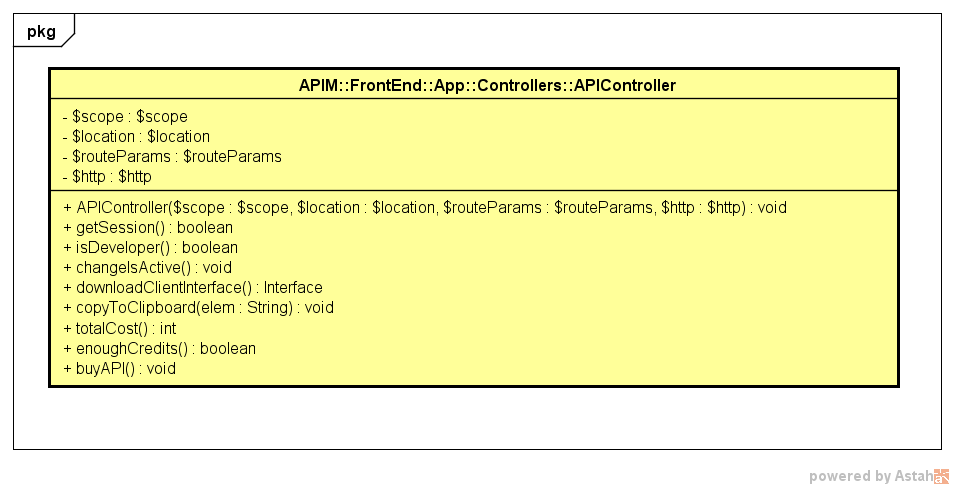
\includegraphics
	[width=0.7\linewidth]
	{images/APIM/FrontEnd/Controllers/APIController.png}
	\caption{APIM::FrontEnd::App::Controllers::APIController}
\end{figure}

\begin{itemize}
	\item \textbf{Descrizione:} APIController permette di ricavare tutte le informazioni riguardanti un'API e di effettuare l'acquisto di una licenza.
	\item \textbf{Attributi:}
	\begin{itemize}
		
		\item \textbf{\$scope : \$scope}\\
		Campo dati contenente un riferimento all'oggetto \$scope creato da AngularJS, viene utilizzato come mezzo di comunicazione tra il controller e la view. Contiene gli oggetti che definiscono il model dell'applicazione;
		
		\item \textbf{\$http : \$http }\\
		Campo dati che contiene un riferimento al servizio \$http che permette la comunicazione con il protocollo HTTP;
		
		\item \textbf{\$location : \$location }\\
		Campo dati contenente il riferimento all'oggetto globale \$location creato da AngularJS. Viene utilizzato per le funzioni di routing;
		
		\item \textbf{\$routeParams : \$routeParams}\\
		Parametro che contiene il riferimento all'oggetto globale \$routeParams di AngularJS. Viene utilizzato per riferirsi alle variabili GET e POST.
		
		
	\end{itemize}
	\item \textbf{Metodi:}
	\begin{itemize}
		
		\item \textbf{APIController(\$scope : \$scope, \$http : \$http, \$location : \$location, \$routeParams : \$routeParams)}\\
		Metodo costruttore della classe;
		\begin{description}
			\item[\textbf{Parametri:}]
		\end{description}
		\begin{itemize}
			\item \textbf{\$scope : \$scope}\\
			Parametro che contiene un riferimento all'oggetto \$scope di AngularJS, impiegato nella comunicazione tra i rispettivi view e controller. Contiene gli oggetti che definiscono i model dell'applicazione;
			
			\item \textbf{\$http : \$http}\\
			Parametro che contiene il riferimento all'oggetto globale \$http di AngularJS. Viene utilizzato per la comunicazione con il protocollo HTTP.
			
			\item \textbf{\$routeParams : \$routeParams}\\
			Parametro che contiene il riferimento all'oggetto globale \$routeParams di AngularJS. Viene utilizzato per riferirsi alle variabili GET e POST.
			
			\item \textbf{\$location : \$location}\\
			Parametro che contiene il riferimento all'oggetto globale \$location di AngularJS. Viene utilizzato per le funzioni di routing.
			
		\end{itemize}		
		
		\item \textbf{isDeveloper() : boolean}\\
		Metodo per verificare se l'utente che sta accedendo ai dati è il developer che la ha registrata;
		\begin{description}
			\item[\textbf{Parametri:}]
		\end{description}
		\begin{itemize}
			\item \textbf{void}\\
		\end{itemize}		
		
		\item \textbf{changeIsActive() : void}\\
		Metodo per attivare lo stato attivo/non attivo dell'API;
		\begin{description}
			\item[\textbf{Parametri:}]
		\end{description}
		\begin{itemize}
			\item \textbf{void}\\
		\end{itemize}		
		
		\item \textbf{downloadClientInterface() : interface}\\
		Metodo per scaricare il file contenente l'interfaccia dell'API;
		\begin{description}
			\item[\textbf{Parametri:}]
		\end{description}
		\begin{itemize}
			\item \textbf{void}\\
		\end{itemize}		
		
		\item \textbf{copyToClipboard(elem : string) : void}\\
		Metodo per copiare le informazioni dell'API;
		\begin{description}
			\item[\textbf{Parametri:}]
		\end{description}
		\begin{itemize}
			\item \textbf{void}\\
		\end{itemize}		
		
		\item \textbf{totalCost() : int}\\
		Metodo per calcolare il costo totale della licenza;
		\begin{description}
			\item[\textbf{Parametri:}]
		\end{description}
		\begin{itemize}
			\item \textbf{void}\\
		\end{itemize}		
		
		\item \textbf{enoughCredits() : boolean}\\
		Metodo per verificare se l'utente che vuole acquistare la licenza ha abbastanza crediti;
		\begin{description}
			\item[\textbf{Parametri:}]
		\end{description}
		\begin{itemize}
			\item \textbf{void}\\
		\end{itemize}		
		
		\item \textbf{buyAPI() : void}\\
		Metodo per verificare effettuare la procedura di acquisto dell'API;
		\begin{description}
			\item[\textbf{Parametri:}]
		\end{description}
		\begin{itemize}
			\item \textbf{void}\\
		\end{itemize}		
		
		
		
	\end{itemize}
	\item \textbf{Relazioni con altre classi:}
	\begin{itemize}
		\item Ricava i dati necessari dal package \textbf{Services};
		\item Gestisce il funzionamento della view \textbf{API};
	\end{itemize}
\end{itemize}

\paragraph{APIM::FrontEnd::App::Controllers::APIListController}

\begin{figure}[H]
	\centering
	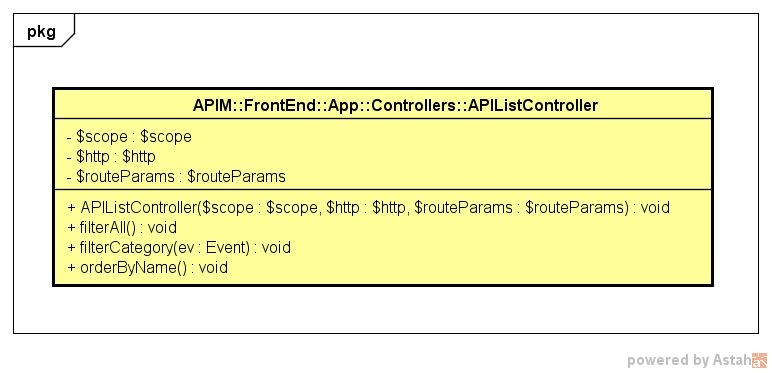
\includegraphics
	[width=0.7\linewidth]
	{images/APIM/FrontEnd/Controllers/APIListController.png}
	\caption{APIM::FrontEnd::App::Controllers::APIListController}
\end{figure}

\begin{itemize}
	\item \textbf{Descrizione:} APIListController permette di ricavare la lista di tutte le API, di ordinare e di filtrare i risultati.
	\item \textbf{Attributi:}
	\begin{itemize}
		
		\item \textbf{\$scope : \$scope}\\
		Campo dati contenente un riferimento all'oggetto \$scope creato da AngularJS, viene utilizzato come mezzo di comunicazione tra il controller e la view. Contiene gli oggetti che definiscono il model dell'applicazione;
		
		\item \textbf{\$http : \$http }\\
		Campo dati che contiene un riferimento al servizio \$http che permette la comunicazione con il protocollo HTTP;
		
		\item \textbf{\$routeParams : \$routeParams}\\
		Parametro che contiene il riferimento all'oggetto globale \$routeParams di AngularJS. Viene utilizzato per riferirsi alle variabili GET e POST.
		
		
	\end{itemize}
	\item \textbf{Metodi:}
	\begin{itemize}
		
		\item \textbf{APIListController(\$scope : \$scope, \$http : \$http, \$routeParams : \$routeParams)}\\
		Metodo costruttore della classe;
		\begin{description}
			\item[\textbf{Parametri:}]
		\end{description}
		\begin{itemize}
			\item \textbf{\$scope : \$scope}\\
			Parametro che contiene un riferimento all'oggetto \$scope di AngularJS, impiegato nella comunicazione tra i rispettivi view e controller. Contiene gli oggetti che definiscono i model dell'applicazione;
			
			\item \textbf{\$http : \$http}\\
			Parametro che contiene il riferimento all'oggetto globale \$http di AngularJS. Viene utilizzato per la comunicazione con il protocollo HTTP.
			
			\item \textbf{\$routeParams : \$routeParams}\\
			Parametro che contiene il riferimento all'oggetto globale \$routeParams di AngularJS. Viene utilizzato per riferirsi alle variabili GET e POST.
			
		\end{itemize}		
		
		\item \textbf{filterAll() : void}\\
		Metodo per visualizzare tutt le categorie;
		\begin{description}
			\item[\textbf{Parametri:}]
		\end{description}
		\begin{itemize}
			\item \textbf{void}\\
		\end{itemize}		
		
		\item \textbf{filterCategory(ev : Event) : void}\\
		Metodo per filtrare solo le categorie selezionate;
		\begin{description}
			\item[\textbf{Parametri:}]
		\end{description}
		\begin{itemize}
			\item \textbf{void}\\
		\end{itemize}		
		
		\item \textbf{orderByName() : void}\\
		Metodo per ordinare le API in modo alfabetico;
		\begin{description}
			\item[\textbf{Parametri:}]
		\end{description}
		\begin{itemize}
			\item \textbf{void}\\
		\end{itemize}		
		
	\end{itemize}
	\item \textbf{Relazioni con altre classi:}
	\begin{itemize}
		\item Ricava i dati necessari dal package \textbf{Services};
		\item Gestisce il funzionamento della view \textbf{APIList};
	\end{itemize}
\end{itemize}

\paragraph{APIM::FrontEnd::App::Controllers::APIPurchasedController}

\begin{figure}[H]
	\centering
	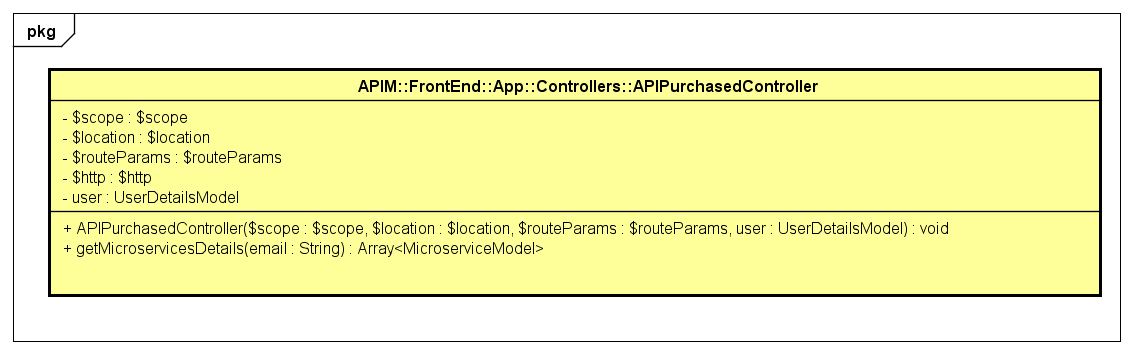
\includegraphics
	[width=0.7\linewidth]
	{images/APIM/FrontEnd/Controllers/APIPurchasedController.png}
	\caption{APIM::FrontEnd::App::Controllers::APIPurchasedController}
\end{figure}

\begin{itemize}
	\item \textbf{Descrizione:} APIPurchasedController permette di vedere lo stato di un API di cui si possiede una licenza.
	\item \textbf{Attributi:}
	\begin{itemize}
		
		\item \textbf{\$scope : \$scope}\\
		Campo dati contenente un riferimento all'oggetto \$scope creato da AngularJS, viene utilizzato come mezzo di comunicazione tra il controller e la view. Contiene gli oggetti che definiscono il model dell'applicazione;
		
		\item \textbf{\$http : \$http }\\
		Campo dati che contiene un riferimento al servizio \$http che permette la comunicazione con il protocollo HTTP;				
		
	\end{itemize}
	\item \textbf{Metodi:}
	\begin{itemize}
		
		\item \textbf{APIPurchasedController(\$scope : \$scope, \$http : \$http)}\\
		Metodo costruttore della classe;
		\begin{description}
			\item[\textbf{Parametri:}]
		\end{description}
		\begin{itemize}
			\item \textbf{\$scope : \$scope}\\
			Parametro che contiene un riferimento all'oggetto \$scope di AngularJS, impiegato nella comunicazione tra i rispettivi view e controller. Contiene gli oggetti che definiscono i model dell'applicazione;
			
			\item \textbf{\$http : \$http}\\
			Parametro che contiene il riferimento all'oggetto globale \$http di AngularJS. Viene utilizzato per la comunicazione con il protocollo HTTP.
			
		\end{itemize}		
		
		\item \textbf{getRemainingSuffix(policyId : int) : void}\\
		Metodo per ricavare la tipologia di policy acquistata;
		\begin{description}
			\item[\textbf{Parametri:}]
		\end{description}
		\begin{itemize}
			\item \textbf{policyId : int}\\
			Idetifica la tipologia di policy.
		\end{itemize}		
		
		\item \textbf{getNewAPIKey(oldAPIKey : String, IdMS : int) : String}\\
		Metodo per generare una nuova API key;
		\begin{description}
			\item[\textbf{Parametri:}]
		\end{description}
		\begin{itemize}
			\item \textbf{oldAPIKey : String}\\
			Vecchia API key;
		\end{itemize}		
		\begin{itemize}
			\item \textbf{IdMS : int}\\
			Identificativo dell'API;
		\end{itemize}		
		
	\end{itemize}
	\item \textbf{Relazioni con altre classi:}
	\begin{itemize}
		\item Ricava i dati necessari dal package \textbf{Services};
		\item Gestisce il funzionamento della view \textbf{APIPurchased};
	\end{itemize}
\end{itemize}

\paragraph{APIM::FrontEnd::App::Controllers::APIRegisteredController}

\begin{figure}[H]
	\centering
	\includegraphics
	[width=0.7\linewidth]
	{images/APIM/FrontEnd/Controllers/APIRegisteredController.png}
	\caption{APIM::FrontEnd::App::Controllers::APIRegisteredController}
\end{figure}

\begin{itemize}
	\item \textbf{Descrizione:} APIRegisteredController permette di ricavare lo stato di un API di cui si ha effettuato la registrazione.
	\item \textbf{Attributi:}
	\begin{itemize}
		
		\item \textbf{\$scope : \$scope}\\
		Campo dati contenente un riferimento all'oggetto \$scope creato da AngularJS, viene utilizzato come mezzo di comunicazione tra il controller e la view. Contiene gli oggetti che definiscono il model dell'applicazione;
		
		\item \textbf{\$rootScope : \$rootScope}\\
		Campo dati contenente un riferimento all'oggetto \$rootScope creato da AngularJS, viene utilizzato come mezzo di comunicazione tra il controller e la view. Contiene gli oggetti che definiscono il model dell'applicazione;
		
		\item \textbf{\$http : \$http }\\
		Campo dati che contiene un riferimento al servizio \$http che permette la comunicazione con il protocollo HTTP;				
		
	\end{itemize}
	\item \textbf{Metodi:}
	\begin{itemize}
		
		\item \textbf{APIRegisteredController(\$scope : \$scope, \$rootScope : \$rootScope, \$http : \$http)}\\
		Metodo costruttore della classe;
		\begin{description}
			\item[\textbf{Parametri:}]
		\end{description}
		\begin{itemize}
			\item \textbf{\$scope : \$scope}\\
			Parametro che contiene un riferimento all'oggetto \$scope di AngularJS, impiegato nella comunicazione tra i rispettivi view e controller. Contiene gli oggetti che definiscono i model dell'applicazione;
			
			\item \textbf{\$rootScope : \$rootScope}\\
			Parametro che contiene un riferimento all'oggetto \$rootScope di AngularJS, impiegato nella comunicazione tra i rispettivi view e controller. Contiene gli oggetti che definiscono i model dell'applicazione;
			
			\item \textbf{\$http : \$http}\\
			Parametro che contiene il riferimento all'oggetto globale \$http di AngularJS. Viene utilizzato per la comunicazione con il protocollo HTTP.
			
		\end{itemize}		
		
	\end{itemize}
	\item \textbf{Relazioni con altre classi:}
	\begin{itemize}
		\item Ricava i dati necessari dal package \textbf{Services};
		\item Gestisce il funzionamento della view \textbf{APIRegistered};
	\end{itemize}
\end{itemize}

\paragraph{APIM::FrontEnd::App::Controllers::CategoryController}

\begin{figure}[H]
	\centering
	\includegraphics
	[width=0.7\linewidth]
	{images/APIM/FrontEnd/Controllers/CategoryController.png}
	\caption{APIM::FrontEnd::App::Controllers::CategoryController}
\end{figure}

\begin{itemize}
	\item \textbf{Descrizione:} CategoryController permette di ricavare le API di una singola categoria.
	\item \textbf{Attributi:}
	\begin{itemize}
		
		\item \textbf{\$scope : \$scope}\\
		Campo dati contenente un riferimento all'oggetto \$scope creato da AngularJS, viene utilizzato come mezzo di comunicazione tra il controller e la view. Contiene gli oggetti che definiscono il model dell'applicazione;
		
		\item \textbf{\$http : \$http }\\
		Campo dati che contiene un riferimento al servizio \$http che permette la comunicazione con il protocollo HTTP;
		
		\item \textbf{\$routeParams : \$routeParams }\\
		Campo dati contenente il riferimento all'oggetto globale \$routeParams creato da AngularJS. Viene utilizzato per riferirsi alle variabili GET e POST;				
		
	\end{itemize}
	\item \textbf{Metodi:}
	\begin{itemize}
		
		\item \textbf{CategoryController(\$scope : \$scope, \$http : \$http, \$routeParams : \$routeParams)}\\
		Metodo costruttore della classe;
		\begin{description}
			\item[\textbf{Parametri:}]
		\end{description}
		\begin{itemize}
			\item \textbf{\$scope : \$scope}\\
			Parametro che contiene un riferimento all'oggetto \$scope di AngularJS, impiegato nella comunicazione tra i rispettivi view e controller. Contiene gli oggetti che definiscono i model dell'applicazione;
			
			\item \textbf{\$http : \$http}\\
			Parametro che contiene il riferimento all'oggetto globale \$http di AngularJS. Viene utilizzato per la comunicazione con il protocollo HTTP.
			
			\item \textbf{\$routeParams : \$routeParams}\\
			Parametro che contiene il riferimento all'oggetto globale \$routeParams di AngularJS. Viene utilizzato per riferirsi alle variabili GET e POST.
			
		\end{itemize}		
		
	\end{itemize}
	\item \textbf{Relazioni con altre classi:}
	\begin{itemize}
		\item Ricava i dati necessari dal package \textbf{Services};
		\item Gestisce il funzionamento della view \textbf{Category};
	\end{itemize}
\end{itemize}

\paragraph{APIM::FrontEnd::App::Controllers::ConfirmAPIRegistrationController}

\begin{figure}[H]
	\centering
	\includegraphics
	[width=0.7\linewidth]
	{images/APIM/FrontEnd/Controllers/ConfirmAPIRegistrationController.png}
	\caption{APIM::FrontEnd::App::Controllers::ConfirmAPIRegistrationController}
\end{figure}

\begin{itemize}
	\item \textbf{Descrizione:} ConfirmAPIRegistrationController permette di effettuare la conferma di registrazione di un API da parte di un utente sviluppatore.
	\item \textbf{Attributi:}
	\begin{itemize}
		
		\item \textbf{\$scope : \$scope}\\
		Campo dati contenente un riferimento all'oggetto \$scope creato da AngularJS, viene utilizzato come mezzo di comunicazione tra il controller e la view. Contiene gli oggetti che definiscono il model dell'applicazione;
		
		\item \textbf{\$http : \$http }\\
		Campo dati che contiene un riferimento al servizio \$http che permette la comunicazione con il protocollo HTTP;
		
		\item \textbf{\$routeParams : \$routeParams }\\
		Campo dati contenente il riferimento all'oggetto globale \$routeParams creato da AngularJS. Viene utilizzato per riferirsi alle variabili GET e POST;				
		
	\end{itemize}
	\item \textbf{Metodi:}
	\begin{itemize}
		
		\item \textbf{ConfirmAPIRegistrationController(\$scope : \$scope, \$http : \$http, \$routeParams : \$routeParams)}\\
		Metodo costruttore della classe;
		\begin{description}
			\item[\textbf{Parametri:}]
		\end{description}
		\begin{itemize}
			\item \textbf{\$scope : \$scope}\\
			Parametro che contiene un riferimento all'oggetto \$scope di AngularJS, impiegato nella comunicazione tra i rispettivi view e controller. Contiene gli oggetti che definiscono i model dell'applicazione;
			
			\item \textbf{\$http : \$http}\\
			Parametro che contiene il riferimento all'oggetto globale \$http di AngularJS. Viene utilizzato per la comunicazione con il protocollo HTTP.
			
			\item \textbf{\$routeParams : \$routeParams}\\
			Parametro che contiene il riferimento all'oggetto globale \$routeParams di AngularJS. Viene utilizzato per riferirsi alle variabili GET e POST.
			
		\end{itemize}		
		
	\end{itemize}
	\item \textbf{Relazioni con altre classi:}
	\begin{itemize}
		\item Ricava i dati necessari dal package \textbf{Services};
		\item Gestisce il funzionamento della view \textbf{ConfirmAPIRegistration};
	\end{itemize}
\end{itemize}

\paragraph{APIM::FrontEnd::App::Controllers::ConfirmUpgradeToDeveloperController}

\begin{figure}[H]
	\centering
	\includegraphics
	[width=0.7\linewidth]
	{images/APIM/FrontEnd/Controllers/ConfirmLoginController.png}
	\caption{APIM::FrontEnd::App::Controllers::ConfirmLoginController}
\end{figure}

\begin{itemize}
	\item \textbf{Descrizione:} ConfirmLoginController permette di confermare l'upgrade da utente cliente a utente sviluppatore.
	\item \textbf{Attributi:}
	\begin{itemize}
		
		\item \textbf{\$scope : \$scope}\\
		Campo dati contenente un riferimento all'oggetto \$scope creato da AngularJS, viene utilizzato come mezzo di comunicazione tra il controller e la view. Contiene gli oggetti che definiscono il model dell'applicazione;
		
		\item \textbf{\$http : \$http }\\
		Campo dati che contiene un riferimento al servizio \$http che permette la comunicazione con il protocollo HTTP;
		
	\end{itemize}
	\item \textbf{Metodi:}
	\begin{itemize}
		
		\item \textbf{ConfirmLoginControllerl(\$scope : \$scope, \$http : \$http)}\\
		Metodo costruttore della classe;
		\begin{description}
			\item[\textbf{Parametri:}]
		\end{description}
		\begin{itemize}
			\item \textbf{\$scope : \$scope}\\
			Parametro che contiene un riferimento all'oggetto \$scope di AngularJS, impiegato nella comunicazione tra i rispettivi view e controller. Contiene gli oggetti che definiscono i model dell'applicazione;
			
			\item \textbf{\$http : \$http}\\
			Parametro che contiene il riferimento all'oggetto globale \$http di AngularJS. Viene utilizzato per la comunicazione con il protocollo HTTP.
			
		\end{itemize}		
		
	\end{itemize}
	\item \textbf{Relazioni con altre classi:}
	\begin{itemize}
		\item Ricava i dati necessari dal package \textbf{Services};
		\item Gestisce il funzionamento della view \textbf{ConfirmUpgradeToDeveloper};
	\end{itemize}
\end{itemize}

\paragraph{APIM::FrontEnd::App::Controllers::ConfirmUserRegistrationController}

\begin{figure}[H]
	\centering
	\includegraphics
	[width=0.7\linewidth]
	{images/APIM/FrontEnd/Controllers/ConfirmUserRegistrationController.png}
	\caption{APIM::FrontEnd::App::Controllers::ConfirmUserRegistrationController}
\end{figure}

\begin{itemize}
	\item \textbf{Descrizione:} ConfirmUserRegistrationController permette di confermare la registrazione di un utente.
	\item \textbf{Attributi:}
	\begin{itemize}
		
		\item \textbf{\$scope : \$scope}\\
		Campo dati contenente un riferimento all'oggetto \$scope creato da AngularJS, viene utilizzato come mezzo di comunicazione tra il controller e la view. Contiene gli oggetti che definiscono il model dell'applicazione;
		
	\end{itemize}
	\item \textbf{Metodi:}
	\begin{itemize}
		
		\item \textbf{ConfirmUserRegistrationController(\$scope : \$scope)}\\
		Metodo costruttore della classe;
		\begin{description}
			\item[\textbf{Parametri:}]
		\end{description}
		\begin{itemize}
			\item \textbf{\$scope : \$scope}\\
			Parametro che contiene un riferimento all'oggetto \$scope di AngularJS, impiegato nella comunicazione tra i rispettivi view e controller. Contiene gli oggetti che definiscono i model dell'applicazione;
			
		\end{itemize}		
		
	\end{itemize}
	\item \textbf{Relazioni con altre classi:}
	\begin{itemize}
		\item Ricava i dati necessari dal package \textbf{Services};
		\item Gestisce il funzionamento della view \textbf{ConfirmUserRegistration};
	\end{itemize}
\end{itemize}

\paragraph{APIM::FrontEnd::App::Controllers::LoginController}

\begin{figure}[H]
	\centering
	\includegraphics
	[width=0.7\linewidth]
	{images/APIM/FrontEnd/Controllers/LoginController.png}
	\caption{APIM::FrontEnd::App::Controllers::LoginController}
\end{figure}

\begin{itemize}
	\item \textbf{Descrizione:} LoginController permette di effettuare il login di clienti e sviluppatori.
	\item \textbf{Attributi:}
	\begin{itemize}
		
		\item \textbf{\$scope : \$scope}\\
		Campo dati contenente un riferimento all'oggetto \$scope creato da AngularJS, viene utilizzato come mezzo di comunicazione tra il controller e la view. Contiene gli oggetti che definiscono il model dell'applicazione;
		
		\item \textbf{\$location : \$location }\\
		Campo dati contenente il riferimento all'oggetto globale \$location creato da AngularJS. Viene utilizzato per riferirsi all'URL ed interagire con il routing;
		
		\item \textbf{\$http : \$http }\\
		Campo dati che contiene un riferimento al servizio \$http che permette la comunicazione con il protocollo HTTP;
		
	\end{itemize}
	\item \textbf{Metodi:}
	\begin{itemize}
		
		\item \textbf{LoginController(\$scope : \$scope, \$location : \$location, \$http : \$http)}\\
		Metodo costruttore della classe;
		\begin{description}
			\item[\textbf{Parametri:}]
		\end{description}
		\begin{itemize}
			\item \textbf{\$scope : \$scope}\\
			Parametro che contiene un riferimento all'oggetto \$scope di AngularJS, impiegato nella comunicazione tra i rispettivi view e controller. Contiene gli oggetti che definiscono i model dell'applicazione;
			
			\item \textbf{\$location : \$location}\\
			Parametro che contiene il riferimento all'oggetto globale \$location di AngularJS. Viene utilizzato per riferirsi all'URL ed interagire con il routing.
			
			\item \textbf{\$http : \$http}\\
			Parametro che contiene il riferimento all'oggetto globale \$http di AngularJS. Viene utilizzato per la comunicazione con il protocollo HTTP.
		\end{itemize}	
		
		\item \textbf{login() : void}\\
		Metodo costruttore della classe;
		\begin{description}
			\item[\textbf{Parametri:}]
		\end{description}
		\begin{itemize}
			\item \textbf{void}\\
		\end{itemize}				
	\end{itemize}
	\item \textbf{Relazioni con altre classi:}
	\begin{itemize}
		\item Ricava i dati necessari dal package \textbf{Services};
		\item Gestisce il funzionamento della view \textbf{Login};
	\end{itemize}
\end{itemize}

\paragraph{APIM::FrontEnd::App::Controllers::LogoutController}

\begin{figure}[H]
	\centering
	\includegraphics
	[width=0.7\linewidth]
	{images/APIM/FrontEnd/Controllers/LogoutController.png}
	\caption{APIM::FrontEnd::App::Controllers::LogoutController}
\end{figure}

\begin{itemize}
	\item \textbf{Descrizione:} LogoutController permette di effettuare il logout di utenti autenticati alla piattaforma.
	\item \textbf{Attributi:}
	\begin{itemize}
		
		\item \textbf{\$scope : \$scope}\\
		Campo dati contenente un riferimento all'oggetto \$scope creato da AngularJS, viene utilizzato come mezzo di comunicazione tra il controller e la view. Contiene gli oggetti che definiscono il model dell'applicazione;
		
		\item \textbf{\$location : \$location }\\
		Campo dati contenente il riferimento all'oggetto globale \$location creato da AngularJS. Viene utilizzato per riferirsi all'URL ed interagire con il routing;
		
	\end{itemize}
	\item \textbf{Metodi:}
	\begin{itemize}
		
		\item \textbf{LogoutController(\$scope : \$scope, \$location : \$location)}\\
		Metodo costruttore della classe;
		\begin{description}
			\item[\textbf{Parametri:}]
		\end{description}
		\begin{itemize}
			\item \textbf{\$scope : \$scope}\\
			Parametro che contiene un riferimento all'oggetto \$scope di AngularJS, impiegato nella comunicazione tra i rispettivi view e controller. Contiene gli oggetti che definiscono i model dell'applicazione;
			
			\item \textbf{\$location : \$location}\\
			Parametro che contiene il riferimento all'oggetto globale \$location di AngularJS. Viene utilizzato per riferirsi all'URL ed interagire con il routing.
			
		\end{itemize}	
					
	\end{itemize}
	\item \textbf{Relazioni con altre classi:}
	\begin{itemize}
		\item Ricava i dati necessari dal package \textbf{Services};
		\item Gestisce il funzionamento della view \textbf{Logout};
	\end{itemize}
\end{itemize}

\paragraph{APIM::FrontEnd::App::Controllers::PasswordRecoveryController}

\begin{figure}[H]
	\centering
	\includegraphics
	[width=0.7\linewidth]
	{images/APIM/FrontEnd/Controllers/PasswordRecoveryController.png}
	\caption{APIM::FrontEnd::App::Controllers::PasswordRecoveryController}
\end{figure}

\begin{itemize}
	\item \textbf{Descrizione:} PasswordRecoveryController permette di effettuare il recupero password di clienti e sviluppatori.
	\item \textbf{Attributi:}
	\begin{itemize}
		
		\item \textbf{\$scope : \$scope}\\
		Campo dati contenente un riferimento all'oggetto \$scope creato da AngularJS, viene utilizzato come mezzo di comunicazione tra il controller e la view. Contiene gli oggetti che definiscono il model dell'applicazione;
		
		\item \textbf{\$http : \$http }\\
		Campo dati che contiene un riferimento al servizio \$http che permette la comunicazione con il protocollo HTTP;
		
	\end{itemize}
	\item \textbf{Metodi:}
	\begin{itemize}
		
		\item \textbf{PasswordRecoveryController(\$scope : \$scope, \$http : \$http)}\\
		Metodo costruttore della classe;
		\begin{description}
			\item[\textbf{Parametri:}]
		\end{description}
		\begin{itemize}
			\item \textbf{\$scope : \$scope}\\
			Parametro che contiene un riferimento all'oggetto \$scope di AngularJS, impiegato nella comunicazione tra i rispettivi view e controller. Contiene gli oggetti che definiscono i model dell'applicazione;
			
			\item \textbf{\$http : \$http}\\
			Parametro che contiene il riferimento all'oggetto globale \$http di AngularJS. Viene utilizzato per la comunicazione con il protocollo HTTP.
			
		\end{itemize}	
		
		\item \textbf{recoverPassword() : void}\\
		Metodo che, attraverso la chiamata all'opportuno microservizio, avvia la procedura di generazione di una nuova password;
		\begin{description}
			\item[\textbf{Parametri:}]
		\end{description}
		\begin{itemize}
			\item \textbf{void}\\
		\end{itemize}				
	\end{itemize}
	\item \textbf{Relazioni con altre classi:}
	\begin{itemize}
		\item Ricava i dati necessari dal package \textbf{Services};
		\item Gestisce il funzionamento della view \textbf{PasswordRecovery};
	\end{itemize}
\end{itemize}

\paragraph{APIM::FrontEnd::App::Controllers::ResetPasswordController}

\begin{figure}[H]
	\centering
	\includegraphics
	[width=0.7\linewidth]
	{images/APIM/FrontEnd/Controllers/ResetPasswordController.png}
	\caption{APIM::FrontEnd::App::Controllers::ResetPasswordController}
\end{figure}

\begin{itemize}
	\item \textbf{Descrizione:} classe che permette di effettuare il cambio password di clienti e sviluppatori autenticati al sistema.
	\item \textbf{Attributi:}
	\begin{itemize}
		
		\item \textbf{\$scope : \$scope}\\
		Campo dati contenente un riferimento all'oggetto \$scope creato da AngularJS, viene utilizzato come mezzo di comunicazione tra il controller e la view. Contiene gli oggetti che definiscono il model dell'applicazione;
		
		\item \textbf{\$http : \$http }\\
		Campo dati che contiene un riferimento al servizio \$http che permette la comunicazione con il protocollo HTTP;
		
		\item \textbf{\$location : \$location}\\
		Parametro che contiene il riferimento all'oggetto globale \$location di AngularJS. Viene utilizzato per riferirsi all'URL ed interagire con il routing.
		
	\end{itemize}
	\item \textbf{Metodi:}
	\begin{itemize}
		
		\item \textbf{ResetPasswordController(\$scope : \$scope, \$http : \$http, \$location : \$location)}\\
		Metodo costruttore della classe;
		\begin{description}
			\item[\textbf{Parametri:}]
		\end{description}
		\begin{itemize}
			\item \textbf{\$scope : \$scope}\\
			Parametro che contiene un riferimento all'oggetto \$scope di AngularJS, impiegato nella comunicazione tra i rispettivi view e controller. Contiene gli oggetti che definiscono i model dell'applicazione;
			
			\item \textbf{\$http : \$http}\\
			Parametro che contiene il riferimento all'oggetto globale \$http di AngularJS. Viene utilizzato per la comunicazione con il protocollo HTTP;
			
			\item \textbf{\$location : \$location}\\
			Parametro che contiene il riferimento all'oggetto globale \$location di AngularJS. Viene utilizzato per riferirsi all'URL ed interagire con il routing.
			
		\end{itemize}	
		
		\item \textbf{changePassword() : void}\\
		Metodo che consente di impostare una nuova password per l'utente;
		\begin{description}
			\item[\textbf{Parametri:}]
		\end{description}
		\begin{itemize}
			\item \textbf{void}\\
		\end{itemize}				
	\end{itemize}
	\item \textbf{Relazioni con altre classi:}
	\begin{itemize}
		\item Ricava i dati necessari dal package \textbf{Services};
		\item Gestisce il funzionamento della view \textbf{ResetPassword};
	\end{itemize}
\end{itemize}

\paragraph{APIM::FrontEnd::App::Controllers::PolicyCallController}

\begin{figure}[H]
	\centering
	\includegraphics
	[width=0.7\linewidth]
	{images/APIM/FrontEnd/Controllers/PolicyCallController.png}
	\caption{APIM::FrontEnd::App::Controllers::PolicyCallController}
\end{figure}

\begin{itemize}
	\item \textbf{Descrizione:} PolicyCallController permette di ricavare le informazioni riguardanti la tipologia di policy a chiamata.
	\item \textbf{Attributi:}
	\begin{itemize}
		
		\item \textbf{\$scope : \$scope}\\
		Campo dati contenente un riferimento all'oggetto \$scope creato da AngularJS, viene utilizzato come mezzo di comunicazione tra il controller e la view. Contiene gli oggetti che definiscono il model dell'applicazione;
		
		\item \textbf{\$http : \$http }\\
		Campo dati che contiene un riferimento al servizio \$http che permette la comunicazione con il protocollo HTTP;
		
	\end{itemize}
	\item \textbf{Metodi:}
	\begin{itemize}
		
		\item \textbf{PolicyCallController(\$scope : \$scope, \$http : \$http)}\\
		Metodo costruttore della classe;
		\begin{description}
			\item[\textbf{Parametri:}]
		\end{description}
		\begin{itemize}
			\item \textbf{\$scope : \$scope}\\
			Parametro che contiene un riferimento all'oggetto \$scope di AngularJS, impiegato nella comunicazione tra i rispettivi view e controller. Contiene gli oggetti che definiscono i model dell'applicazione;
			
			\item \textbf{\$http : \$http}\\
			Parametro che contiene il riferimento all'oggetto globale \$http di AngularJS. Viene utilizzato per la comunicazione con il protocollo HTTP.
			
		\end{itemize}				
	\end{itemize}
	\item \textbf{Relazioni con altre classi:}
	\begin{itemize}
		\item Ricava i dati necessari dal package \textbf{Services};
		\item Gestisce il funzionamento della view \textbf{PolicyCall};
	\end{itemize}
\end{itemize}

\paragraph{APIM::FrontEnd::App::Controllers::PolicyTimeController}

\begin{figure}[H]
	\centering
	\includegraphics
	[width=0.7\linewidth]
	{images/APIM/FrontEnd/Controllers/PolicyTimeController.png}
	\caption{APIM::FrontEnd::App::Controllers::PolicyTimeController}
\end{figure}

\begin{itemize}
	\item \textbf{Descrizione:} PolicyTimeController permette di ricavare le informazioni riguardanti la tipologia di policy a tempo.
	\item \textbf{Attributi:}
	\begin{itemize}
		
		\item \textbf{\$scope : \$scope}\\
		Campo dati contenente un riferimento all'oggetto \$scope creato da AngularJS, viene utilizzato come mezzo di comunicazione tra il controller e la view. Contiene gli oggetti che definiscono il model dell'applicazione;
		
		\item \textbf{\$http : \$http }\\
		Campo dati che contiene un riferimento al servizio \$http che permette la comunicazione con il protocollo HTTP;
		
	\end{itemize}
	\item \textbf{Metodi:}
	\begin{itemize}
		
		\item \textbf{PolicyTimeController(\$scope : \$scope, \$http : \$http)}\\
		Metodo costruttore della classe;
		\begin{description}
			\item[\textbf{Parametri:}]
		\end{description}
		\begin{itemize}
			\item \textbf{\$scope : \$scope}\\
			Parametro che contiene un riferimento all'oggetto \$scope di AngularJS, impiegato nella comunicazione tra i rispettivi view e controller. Contiene gli oggetti che definiscono i model dell'applicazione;
			
			\item \textbf{\$http : \$http}\\
			Parametro che contiene il riferimento all'oggetto globale \$http di AngularJS. Viene utilizzato per la comunicazione con il protocollo HTTP.
			
		\end{itemize}				
	\end{itemize}
	\item \textbf{Relazioni con altre classi:}
	\begin{itemize}
		\item Ricava i dati necessari dal package \textbf{Services};
		\item Gestisce il funzionamento della view \textbf{PolicyTime};
	\end{itemize}
\end{itemize}

\paragraph{APIM::FrontEnd::App::Controllers::PolicyTrafficController}

\begin{figure}[H]
	\centering
	\includegraphics
	[width=0.7\linewidth]
	{images/APIM/FrontEnd/Controllers/PolicyTrafficController.png}
	\caption{APIM::FrontEnd::App::Controllers::PolicyTrafficController}
\end{figure}

\begin{itemize}
	\item \textbf{Descrizione:} PolicyTrafficController permette di ricavare le informazioni riguardanti la tipologia di policy a traffico dati.
	\item \textbf{Attributi:}
	\begin{itemize}
		
		\item \textbf{\$scope : \$scope}\\
		Campo dati contenente un riferimento all'oggetto \$scope creato da AngularJS, viene utilizzato come mezzo di comunicazione tra il controller e la view. Contiene gli oggetti che definiscono il model dell'applicazione;
		
		\item \textbf{\$http : \$http }\\
		Campo dati che contiene un riferimento al servizio \$http che permette la comunicazione con il protocollo HTTP;
		
	\end{itemize}
	\item \textbf{Metodi:}
	\begin{itemize}
		
		\item \textbf{PolicyTrafficController(\$scope : \$scope, \$http : \$http)}\\
		Metodo costruttore della classe;
		\begin{description}
			\item[\textbf{Parametri:}]
		\end{description}
		\begin{itemize}
			\item \textbf{\$scope : \$scope}\\
			Parametro che contiene un riferimento all'oggetto \$scope di AngularJS, impiegato nella comunicazione tra i rispettivi view e controller. Contiene gli oggetti che definiscono i model dell'applicazione;
			
			\item \textbf{\$http : \$http}\\
			Parametro che contiene il riferimento all'oggetto globale \$http di AngularJS. Viene utilizzato per la comunicazione con il protocollo HTTP.
			
		\end{itemize}				
	\end{itemize}
	\item \textbf{Relazioni con altre classi:}
	\begin{itemize}
		\item Ricava i dati necessari dal package \textbf{Services};
		\item Gestisce il funzionamento della view \textbf{PolicyTraffic};
	\end{itemize}
\end{itemize}

\paragraph{APIM::FrontEnd::App::Controllers::ProfileManagerController}

\begin{figure}[H]
	\centering
	\includegraphics
	[width=0.7\linewidth]
	{images/APIM/FrontEnd/Controllers/ProfileManagerController.png}
	\caption{APIM::FrontEnd::App::Controllers::ProfileManagerController}
\end{figure}

\begin{itemize}
	\item \textbf{Descrizione:} ProfileManagerController permette di gestire il profilo personale di un
	utente, fornendogli le funzionalità per poter modificare i propri dati.
	\item \textbf{Attributi:}
	\begin{itemize}
		
		\item \textbf{\$scope : \$scope}\\
		Campo dati contenente un riferimento all'oggetto \$scope creato da AngularJS, viene utilizzato come mezzo di comunicazione tra il controller e la view. Contiene gli oggetti che definiscono il model dell'applicazione;
		
		\item \textbf{\$window : \$window}\\
		Campo dati contenente il riferimento all'oggetto globale \$window creato da AngularJS. Viene utilizzato per riferisi all'oggetto window del browser;
		
		\item \textbf{\$location : \$location }\\
		Campo dati contenente il riferimento all'oggetto globale \$location creato da AngularJS. Viene utilizzato per riferirsi all'URL ed interagire con il routing;
		
		\item \textbf{\$http : \$http }\\
		Campo dati che contiene un riferimento al servizio \$http che permette la comunicazione con il protocollo HTTP;
		
		
	\end{itemize}
	\item \textbf{Metodi:}
	\begin{itemize}
		
		\item \textbf{ProfileManagerController(\$scope : \$scope, \$location : \$location, \$http : \$http, \$window : \$window,}\\
		Metodo costruttore della classe;
		\begin{description}
			\item[\textbf{Parametri:}]
		\end{description}
		\begin{itemize}
			\item \textbf{\$scope : \$scope}\\
			Parametro che contiene un riferimento all'oggetto \$scope di AngularJS, impiegato nella comunicazione tra i rispettivi view e controller. Contiene gli oggetti che definiscono i model dell'applicazione;
			
			\item \textbf{\$location : \$location}\\
			Parametro che contiene il riferimento all'oggetto globale \$location di AngularJS. Viene utilizzato per riferirsi all'URL ed interagire con il routing.
			
			\item \textbf{\$http : \$http}\\
			Parametro che contiene il riferimento all'oggetto globale \$http di AngularJS. Viene utilizzato per la comunicazione con il protocollo HTTP.
			
			\item \textbf{\$window : \$window}\\
			Parametro che contiene il riferimento all'oggetto globale \$window di AngularJS. Viene utilizzato per interagire con l'oggeto window del browser.
		\end{itemize}
		
		\item \textbf{updateProfile() : void}\\
		Metodo per aggiornare i dati del profilo utente. Si serve di un'operazione di un servizio esposto dal package \textbf{Services}.
		\begin{description}
			\item[\textbf{Parametri:}]
		\end{description}
		\begin{itemize}
			\item \textbf{void}\\
		\end{itemize}
		
		\item \textbf{updateAvatar(element : Image) : void}\\
		Metodo per modificare l'avatar del profilo utente. Si serve di un'operazione di un servizio esposto dal package \textbf{Services}.
		\begin{description}
			\item[\textbf{Parametri:}]
		\end{description}
		\begin{itemize}
			\item \textbf{element : Image}\\
			Parametro che rappresenta l'immagine avatar dell'utente.
		\end{itemize}
		
	\end{itemize}
	\item \textbf{Relazioni con altre classi:}
	\begin{itemize}
		\item Ricava i dati necessari dal package \textbf{Services};
		\item Gestisce il funzionamento della view \textbf{ProfileManager};
		\item Il model \textbf{UsersDetailModel} che contiene le informazioni per rappresentare un utente.
	\end{itemize}
\end{itemize}

\paragraph{APIM::FrontEnd::App::Controllers::RechargedCreditsController}

\begin{figure}[H]
	\centering
	\includegraphics
	[width=0.7\linewidth]
	{images/APIM/FrontEnd/Controllers/RechargeCreditsController.png}
	\caption{APIM::FrontEnd::App::Controllers::RechargeCreditsController}
\end{figure}

\begin{itemize}
	\item \textbf{Descrizione:} RechargeCreditsController permette di effettuare la ricarica di crediti nel profilo di clienti e sviluppatori.
	\item \textbf{Attributi:}
	\begin{itemize}
		
		\item \textbf{\$scope : \$scope}\\
		Campo dati contenente un riferimento all'oggetto \$scope creato da AngularJS, viene utilizzato come mezzo di comunicazione tra il controller e la view. Contiene gli oggetti che definiscono il model dell'applicazione;
		
		\item \textbf{\$location : \$location }\\
		Campo dati contenente il riferimento all'oggetto globale \$location creato da AngularJS. Viene utilizzato per riferirsi all'URL ed interagire con il routing;
		
		\item \textbf{\$http : \$http }\\
		Campo dati che contiene un riferimento al servizio \$http che permette la comunicazione con il protocollo HTTP;
		
	\end{itemize}
	\item \textbf{Metodi:}
	\begin{itemize}
		
		\item \textbf{RechargeCreditsController(\$scope : \$scope, \$location : \$location, \$http : \$http)}\\
		Metodo costruttore della classe;
		\begin{description}
			\item[\textbf{Parametri:}]
		\end{description}
		\begin{itemize}
			\item \textbf{\$scope : \$scope}\\
			Parametro che contiene un riferimento all'oggetto \$scope di AngularJS, impiegato nella comunicazione tra i rispettivi view e controller. Contiene gli oggetti che definiscono i model dell'applicazione;
			
			\item \textbf{\$location : \$location}\\
			Parametro che contiene il riferimento all'oggetto globale \$location di AngularJS. Viene utilizzato per riferirsi all'URL ed interagire con il routing.
			
			\item \textbf{\$http : \$http}\\
			Parametro che contiene il riferimento all'oggetto globale \$http di AngularJS. Viene utilizzato per la comunicazione con il protocollo HTTP.
		\end{itemize}				
		
	\end{itemize}
	\item \textbf{Relazioni con altre classi:}
	\begin{itemize}
		\item Ricava i dati necessari dal package \textbf{Services};
		\item Gestisce il funzionamento della view \textbf{RechargeCredits};
	\end{itemize}
\end{itemize}

\paragraph{APIM::FrontEnd::App::Controllers::RegisterAPIController}

\begin{figure}[H]
	\centering
	\includegraphics
	[width=0.7\linewidth]
	{images/APIM/FrontEnd/Controllers/RegisterAPIController.png}
	\caption{APIM::FrontEnd::App::Controllers::RegisterAPIController}
\end{figure}

\begin{itemize}
	\item \textbf{Descrizione:} RegisterAPIController permette di effettuare tutte le operazioni per la registrazione di un API.
	\item \textbf{Attributi:}
	\begin{itemize}
		
		\item \textbf{\$scope : \$scope}\\
		Campo dati contenente un riferimento all'oggetto \$scope creato da AngularJS, viene utilizzato come mezzo di comunicazione tra il controller e la view. Contiene gli oggetti che definiscono il model dell'applicazione;
		
		\item \textbf{\$window : \$window}\\
		Campo dati contenente il riferimento all'oggetto globale \$window creato da AngularJS. Viene utilizzato per riferisi all'oggetto window del browser;
		
		\item \textbf{\$location : \$location }\\
		Campo dati contenente il riferimento all'oggetto globale \$location creato da AngularJS. Viene utilizzato per riferirsi all'URL ed interagire con il routing;
		
		\item \textbf{\$http : \$http }\\
		Campo dati che contiene un riferimento al servizio \$http che permette la comunicazione con il protocollo HTTP;
		
		
	\end{itemize}
	\item \textbf{Metodi:}
	\begin{itemize}
		
		\item \textbf{RegisterAPIController(\$scope : \$scope, \$location : \$location, \$http : \$http, \$window : \$window,}\\
		Metodo costruttore della classe;
		\begin{description}
			\item[\textbf{Parametri:}]
		\end{description}
		\begin{itemize}
			\item \textbf{\$scope : \$scope}\\
			Parametro che contiene un riferimento all'oggetto \$scope di AngularJS, impiegato nella comunicazione tra i rispettivi view e controller. Contiene gli oggetti che definiscono i model dell'applicazione;
			
			\item \textbf{\$location : \$location}\\
			Parametro che contiene il riferimento all'oggetto globale \$location di AngularJS. Viene utilizzato per riferirsi all'URL ed interagire con il routing.
			
			\item \textbf{\$http : \$http}\\
			Parametro che contiene il riferimento all'oggetto globale \$http di AngularJS. Viene utilizzato per la comunicazione con il protocollo HTTP.
			
			\item \textbf{\$window : \$window}\\
			Parametro che contiene il riferimento all'oggetto globale \$window di AngularJS. Viene utilizzato per interagire con l'oggeto window del browser.
		\end{itemize}
		
		\item \textbf{addNewSubService() : boolean}\\
		Metodo per aggiungere il riferimento ad un subservizio. Si serve di un'operazione di un servizio esposto dal package \textbf{Services}.
		\begin{description}
			\item[\textbf{Parametri:}]
		\end{description}
		\begin{itemize}
			\item \textbf{void}\\
		\end{itemize}
		
		\item \textbf{removeSubService() : boolean}\\
		Metodo per eliminare il riferimento ad un subservizio. Si serve di un'operazione di un servizio esposto dal package \textbf{Services}.
		\begin{description}
			\item[\textbf{Parametri:}]
		\end{description}
		\begin{itemize}
			\item \textbf{void}\\
		\end{itemize}
		
		\item \textbf{saveInterface(element : Interface) : void}\\
		Metodo per aggiungere il file di interfaccia del subservizio. Si serve di un'operazione di un servizio esposto dal package \textbf{Services}.
		\begin{description}
			\item[\textbf{Parametri:}]
		\end{description}
		\begin{itemize}
			\item \textbf{element : Interface}\\
			File di interfaccia del servizio.
		\end{itemize}
		
		\item \textbf{uploadPDF(element : PDF) : void}\\
		Metodo per aggiungere il file di documentazione in formato PDF. Si serve di un'operazione di un servizio esposto dal package \textbf{Services}.
		\begin{description}
			\item[\textbf{Parametri:}]
		\end{description}
		\begin{itemize}
			\item \textbf{element : PDF}\\
			File di documentazione del servizio.
		\end{itemize}
		
		\item \textbf{uploadLogo(element : Image) : void}\\
		Metodo per aggiungere il logo. Si serve di un'operazione di un servizio esposto dal package \textbf{Services}.
		\begin{description}
			\item[\textbf{Parametri:}]
		\end{description}
		\begin{itemize}
			\item \textbf{element : Image}\\
			File imagine del logo del servizio.
		\end{itemize}
		
		\item \textbf{submit() : void}\\
		Metodo per effettuare la registrazione dell'API. Si serve di un'operazione di un servizio esposto dal package \textbf{Services}.
		\begin{description}
			\item[\textbf{Parametri:}]
		\end{description}
		\begin{itemize}
			\item \textbf{void}\\
		\end{itemize}
		
	\end{itemize}
	\item \textbf{Relazioni con altre classi:}
	\begin{itemize}
		\item Ricava i dati necessari dal package \textbf{Services};
		\item Gestisce il funzionamento della view \textbf{RegisterAPI};
	\end{itemize}
\end{itemize}

\paragraph{APIM::FrontEnd::App::Controllers::RegisterUserController}

\begin{figure}[H]
	\centering
	\includegraphics
	[width=0.7\linewidth]
	{images/APIM/FrontEnd/Controllers/RegisterUserController.png}
	\caption{APIM::FrontEnd::App::Controllers::RegisterUserController}
\end{figure}

\begin{itemize}
	\item \textbf{Descrizione:} RegisterUserController permette di effettuare la registrazione di un utente.
	\item \textbf{Attributi:}
	\begin{itemize}
		
		\item \textbf{\$scope : \$scope}\\
		Campo dati contenente un riferimento all'oggetto \$scope creato da AngularJS, viene utilizzato come mezzo di comunicazione tra il controller e la view. Contiene gli oggetti che definiscono il model dell'applicazione;
		
		\item \textbf{\$window : \$window}\\
		Campo dati contenente il riferimento all'oggetto globale \$window creato da AngularJS. Viene utilizzato per riferisi all'oggetto window del browser;
		
		\item \textbf{\$location : \$location }\\
		Campo dati contenente il riferimento all'oggetto globale \$location creato da AngularJS. Viene utilizzato per riferirsi all'URL ed interagire con il routing;
		
		\item \textbf{\$http : \$http }\\
		Campo dati che contiene un riferimento al servizio \$http che permette la comunicazione con il protocollo HTTP;
		
		
	\end{itemize}
	\item \textbf{Metodi:}
	\begin{itemize}
		
		\item \textbf{RegisterUserController(\$scope : \$scope, \$location : \$location, \$http : \$http, \$window : \$window,}\\
		Metodo costruttore della classe;
		\begin{description}
			\item[\textbf{Parametri:}]
		\end{description}
		\begin{itemize}
			\item \textbf{\$scope : \$scope}\\
			Parametro che contiene un riferimento all'oggetto \$scope di AngularJS, impiegato nella comunicazione tra i rispettivi view e controller. Contiene gli oggetti che definiscono i model dell'applicazione;
			
			\item \textbf{\$location : \$location}\\
			Parametro che contiene il riferimento all'oggetto globale \$location di AngularJS. Viene utilizzato per riferirsi all'URL ed interagire con il routing.
			
			\item \textbf{\$http : \$http}\\
			Parametro che contiene il riferimento all'oggetto globale \$http di AngularJS. Viene utilizzato per la comunicazione con il protocollo HTTP.
			
			\item \textbf{\$window : \$window}\\
			Parametro che contiene il riferimento all'oggetto globale \$window di AngularJS. Viene utilizzato per interagire con l'oggeto window del browser.
		\end{itemize}
		
		\item \textbf{submitForm() : void}\\
		Invia il form con i dati per la registrazione. Si serve di un'operazione di un servizio esposto dal package \textbf{Services}.
		\begin{description}
			\item[\textbf{Parametri:}]
		\end{description}
		\begin{itemize}
			\item \textbf{void}\\
		\end{itemize}
		
		\item \textbf{updloadAvatar(element : Image) : void}\\
		Metodo per caricare l'avatar del profilo utente. Si serve di un'operazione di un servizio esposto dal package \textbf{Services}.
		\begin{description}
			\item[\textbf{Parametri:}]
		\end{description}
		\begin{itemize}
			\item \textbf{element : Image}\\
			Parametro che rappresenta un indirizzo email.
		\end{itemize}
		
	\end{itemize}
	\item \textbf{Relazioni con altre classi:}
	\begin{itemize}
		\item Ricava i dati necessari dal package \textbf{Services};
		\item Gestisce il funzionamento della view \textbf{RegisterUser};
	\end{itemize}
\end{itemize}

\paragraph{APIM::FrontEnd::App::Controllers::ShowUserDetailController}

\begin{figure}[H]
	\centering
	\includegraphics
	[width=0.7\linewidth]
	{images/APIM/FrontEnd/Controllers/ShowUserDetailsController.png}
	\caption{APIM::FrontEnd::App::Controllers::ShowUserDetailsController}
\end{figure}

\begin{itemize}
	\item \textbf{Descrizione:} ShowUserDetailsController permette di ricavare le informazioni di un utente.
	\item \textbf{Attributi:}
	\begin{itemize}
		
		\item \textbf{\$scope : \$scope}\\
		Campo dati contenente un riferimento all'oggetto \$scope creato da AngularJS, viene utilizzato come mezzo di comunicazione tra il controller e la view. Contiene gli oggetti che definiscono il model dell'applicazione;
		
		\item \textbf{\$http : \$http }\\
		Campo dati che contiene un riferimento al servizio \$http che permette la comunicazione con il protocollo HTTP;
		
		\item \textbf{\$routeParams : \$routeParams }\\
		Campo dati contenente il riferimento all'oggetto globale \$routeParams creato da AngularJS. Viene utilizzato per riferirsi alle variabili GET e POST;	
		
	\end{itemize}
	\item \textbf{Metodi:}
	\begin{itemize}
		
		\item \textbf{ShowUserDetailsController(\$scope : \$scope, \$http : \$http, \$routeParams : \$routeParams,}\\
		Metodo costruttore della classe;
		\begin{description}
			\item[\textbf{Parametri:}]
		\end{description}
		\begin{itemize}
			\item \textbf{\$scope : \$scope}\\
			Parametro che contiene un riferimento all'oggetto \$scope di AngularJS, impiegato nella comunicazione tra i rispettivi view e controller. Contiene gli oggetti che definiscono i model dell'applicazione;
			
			\item \textbf{\$http : \$http}\\
			Parametro che contiene il riferimento all'oggetto globale \$http di AngularJS. Viene utilizzato per la comunicazione con il protocollo HTTP.
			
			\item \textbf{\$routeParams : \$routeParams}\\
			Parametro che contiene il riferimento all'oggetto globale \$routeParams di AngularJS. Viene utilizzato per riferirsi alle variabili GET e POST.
			
		\end{itemize}
		
	\end{itemize}
	\item \textbf{Relazioni con altre classi:}
	\begin{itemize}
		\item Ricava i dati necessari dal package \textbf{Services};
		\item Gestisce il funzionamento della view \textbf{ShowUserDetails};
	\end{itemize}
\end{itemize}

\paragraph{APIM::FrontEnd::App::Controllers::TransactionsListController}

\begin{figure}[H]
	\centering
	\includegraphics
	[width=0.7\linewidth]
	{images/APIM/FrontEnd/Controllers/TransactionsListController.png}
	\caption{APIM::FrontEnd::App::Controllers::TransactionsListController}
\end{figure}

\begin{itemize}
	\item \textbf{Descrizione:} TransactionsListController permette di ricavare la lista delle transazioni per un utente.
	\item \textbf{Attributi:}
	\begin{itemize}
		
		\item \textbf{\$scope : \$scope}\\
		Campo dati contenente un riferimento all'oggetto \$scope creato da AngularJS, viene utilizzato come mezzo di comunicazione tra il controller e la view. Contiene gli oggetti che definiscono il model dell'applicazione;
		
		\item \textbf{\$http : \$http }\\
		Campo dati che contiene un riferimento al servizio \$http che permette la comunicazione con il protocollo HTTP;
		
	\end{itemize}
	\item \textbf{Metodi:}
	\begin{itemize}
		
		\item \textbf{TransactionsListController(\$scope : \$scope, \$http : \$http, \$routeParams : \$routeParams,}\\
		Metodo costruttore della classe;
		\begin{description}
			\item[\textbf{Parametri:}]
		\end{description}
		\begin{itemize}
			\item \textbf{\$scope : \$scope}\\
			Parametro che contiene un riferimento all'oggetto \$scope di AngularJS, impiegato nella comunicazione tra i rispettivi view e controller. Contiene gli oggetti che definiscono i model dell'applicazione;
			
			\item \textbf{\$http : \$http}\\
			Parametro che contiene il riferimento all'oggetto globale \$http di AngularJS. Viene utilizzato per la comunicazione con il protocollo HTTP.
			
		\end{itemize}
		
	\end{itemize}
	\item \textbf{Relazioni con altre classi:}
	\begin{itemize}
		\item Ricava i dati necessari dal package \textbf{Services};
		\item Gestisce il funzionamento della view \textbf{TransactionsList};
	\end{itemize}
\end{itemize}

\paragraph{APIM::FrontEnd::App::Controllers::UpdateInfoAPIController}

\begin{figure}[H]
	\centering
	\includegraphics
	[width=0.7\linewidth]
	{images/APIM/FrontEnd/Controllers/UpdateInfoAPIController.png}
	\caption{APIM::FrontEnd::App::Controllers::UpdateInfoAPIController}
\end{figure}

\begin{itemize}
	\item \textbf{Descrizione:} UpdateInfoAPIController permette di effettuare tutte le operazioni per l'aggiornamento delle informazioni di una API.
	\item \textbf{Attributi:}
	\begin{itemize}
		
		\item \textbf{\$scope : \$scope}\\
		Campo dati contenente un riferimento all'oggetto \$scope creato da AngularJS, viene utilizzato come mezzo di comunicazione tra il controller e la view. Contiene gli oggetti che definiscono il model dell'applicazione;
		
		\item \textbf{\$http : \$http }\\
		Campo dati che contiene un riferimento al servizio \$http che permette la comunicazione con il protocollo HTTP;
		
		\item \textbf{\$routeParams : \$routeParams }\\
		Campo dati contenente il riferimento all'oggetto globale \$routeParams creato da AngularJS. Viene utilizzato per riferirsi alle variabili GET e POST;	
		
	\end{itemize}
	\item \textbf{Metodi:}
	\begin{itemize}
		
		\item \textbf{UpdateInfoAPIController(\$scope : \$scope, \$location : \$location, \$http : \$http, \$window : \$window,}\\
		Metodo costruttore della classe;
		\begin{description}
			\item[\textbf{Parametri:}]
		\end{description}
		\begin{itemize}
			\item \textbf{\$scope : \$scope}\\
			Parametro che contiene un riferimento all'oggetto \$scope di AngularJS, impiegato nella comunicazione tra i rispettivi view e controller. Contiene gli oggetti che definiscono i model dell'applicazione;
			
			\item \textbf{\$http : \$http}\\
			Parametro che contiene il riferimento all'oggetto globale \$http di AngularJS. Viene utilizzato per la comunicazione con il protocollo HTTP.
			
			\item \textbf{\$routeParams : \$routeParams}\\
			Parametro che contiene il riferimento all'oggetto globale \$routeParams di AngularJS. Viene utilizzato per riferirsi alle variabili GET e POST.
		\end{itemize}
		
		\item \textbf{addNewCategory(event : Category) : void}\\
		Metodo per aggiungere l'API alla categoria selezionata. Si serve di un'operazione di un servizio esposto dal package \textbf{Services}.
		\begin{description}
			\item[\textbf{Parametri:}]
		\end{description}
		\begin{itemize}
			\item \textbf{event : Category}\\
			Categoria a cui aggiungere l'API.
		\end{itemize}
		
		\item \textbf{updateCategories() : void}\\
		Metodo per aggiornare le categorie associate all'API. Si serve di un'operazione di un servizio esposto dal package \textbf{Services}.
		\begin{description}
			\item[\textbf{Parametri:}]
		\end{description}
		\begin{itemize}
			\item \textbf{void}\\
		\end{itemize}
		
		\item \textbf{uploadPDF(element : PDF) : void}\\
		Metodo per aggiungere il file di documentazione in formato PDF. Si serve di un'operazione di un servizio esposto dal package \textbf{Services}.
		\begin{description}
			\item[\textbf{Parametri:}]
		\end{description}
		\begin{itemize}
			\item \textbf{element : PDF}\\
			File di documentazione del microservizio.
		\end{itemize}
		
		\item \textbf{uploadLogo(element : Image) : void}\\
		Metodo per aggiungere il logo di un microservizio. Si serve di un'operazione di un servizio esposto dal package \textbf{Services}.
		\begin{description}
			\item[\textbf{Parametri:}]
		\end{description}
		\begin{itemize}
			\item \textbf{element : Image}\\
			File immagine del logo del microservizio.
		\end{itemize}
		
		\item \textbf{submit() : void}\\
		Metodo per effettuare l'invio e la modifica delle nuove informazioni per l'API selezionata. Si serve di un'operazione di un servizio esposto dal package \textbf{Services}.
		\begin{description}
			\item[\textbf{Parametri:}]
		\end{description}
		\begin{itemize}
			\item \textbf{void}\\
		\end{itemize}
		
		\item \textbf{changeIsActive() : void}\\
		Metodo per effettuare la commutazione dello stato (attivo/non attivo) dell'API. Si serve di un'operazione di un servizio esposto dal package \textbf{Services}.
		\begin{description}
			\item[\textbf{Parametri:}]
		\end{description}
		\begin{itemize}
			\item \textbf{void}\\
		\end{itemize}
		
	\end{itemize}
	\item \textbf{Relazioni con altre classi:}
	\begin{itemize}
		\item Ricava i dati necessari dal package \textbf{Services};
		\item Gestisce il funzionamento della view \textbf{UpdateInfoAPI};
	\end{itemize}
\end{itemize}

\paragraph{APIM::FrontEnd::App::Controllers::UpgradeToDeveloperController}

\begin{figure}[H]
	\centering
	\includegraphics
	[width=0.7\linewidth]
	{images/APIM/FrontEnd/Controllers/UpgradeToDeveloperController.png}
	\caption{APIM::FrontEnd::App::Controllers::UpgradeToDeveloperController}
\end{figure}

\begin{itemize}
	\item \textbf{Descrizione:} UpgradeToDeveloperController permette di effettuare l'aggiornamento di un cliente allo stato di sviluppatore.
	\item \textbf{Attributi:}
	\begin{itemize}
		
		\item \textbf{\$scope : \$scope}\\
		Campo dati contenente un riferimento all'oggetto \$scope creato da AngularJS, viene utilizzato come mezzo di comunicazione tra il controller e la view. Contiene gli oggetti che definiscono il model dell'applicazione;
		
		\item \textbf{\$http : \$http }\\
		Campo dati che contiene un riferimento al servizio \$http che permette la comunicazione con il protocollo HTTP;
		
		\item \textbf{\$location : \$location }\\
		Campo dati contenente il riferimento all'oggetto globale \$location creato da AngularJS. Viene utilizzato per le funzioni di routing;
		
		
	\end{itemize}
	\item \textbf{Metodi:}
	\begin{itemize}
		
		\item \textbf{UpgradeToDeveloperController(\$scope : \$scope, \$http : \$http, \$location : \$location)}\\
		Metodo costruttore della classe;
		\begin{description}
			\item[\textbf{Parametri:}]
		\end{description}
		\begin{itemize}
			\item \textbf{\$scope : \$scope}\\
			Parametro che contiene un riferimento all'oggetto \$scope di AngularJS, impiegato nella comunicazione tra i rispettivi view e controller. Contiene gli oggetti che definiscono i model dell'applicazione;
			
			\item \textbf{\$http : \$http}\\
			Parametro che contiene il riferimento all'oggetto globale \$http di AngularJS. Viene utilizzato per la comunicazione con il protocollo HTTP.
			
			\item \textbf{\$location : \$location}\\
			Parametro che contiene il riferimento all'oggetto globale \$location di AngularJS. Viene utilizzato per le funzioni di routing.
			
		\end{itemize}
		
		\item \textbf{enoughCredits() : boolean}\\
		Metodo che verifica se il cliente possiede abbastanza crediti per effettuare l'upgrade. Si serve di un'operazione di un servizio esposto dal package \textbf{Services}.
		\begin{description}
			\item[\textbf{Parametri:}]
		\end{description}
		\begin{itemize}
			\item \textbf{void}\\
		\end{itemize}
		
		\item \textbf{developerUpgrade() : void}\\
		Metodo che effettua l'upgrade dell'utente. Si serve di un'operazione di un servizio esposto dal package \textbf{Services}.
		\begin{description}
			\item[\textbf{Parametri:}]
		\end{description}
		\begin{itemize}
			\item \textbf{void}\\
		\end{itemize}
		
		
		
	\end{itemize}
	\item \textbf{Relazioni con altre classi:}
	\begin{itemize}
		\item Ricava i dati necessari dal package \textbf{Services};
		\item Gestisce il funzionamento della view \textbf{UpgradeToDeveloper};
	\end{itemize}
\end{itemize}

% Fine controllers

\subsection{APIM::FrontEnd::App::node\_modules}

\subsubsection{Informazioni generali}

\begin{figure}[H]
	\centering
	\includegraphics
	[width=0.7\linewidth]
	{images/APIM/FrontEnd/NodeModules.png}
	\caption{APIM::FrontEnd::App::node\_modules}
\end{figure}

\begin{itemize}
	\item \textbf{Descrizione:} Il package \textit{node\_modules} contiene tutti i moduli che Node.js mette a disposizione e che possono essere utilizzati dall'applicazione web.
\end{itemize}

%fine node modules